\subsection{Effective rank of power series kernels}
Recall that for a positive semidefinite matrix $\Ab$ we define the \textit{effective rank} \cite{DBLP:journals/simods/HuangHV22} via the following ratio
\[ \mathrm{eff}(\Ab) := \frac{Tr(\Ab)}{\lambda_1(\Ab)}. \]
We consider a kernel Gram matrix $\mK \in \mathbb{R}^{n \times n}$ that has the following power series representation in terms of an input gram matrix $\mX \mX^T$
\[ n \mK = \sum_{i = 0}^\infty c_i (\mX \mX^T)^{\odot i}. \]
Whenever $c_0 \neq 0$ the effective rank of $\mK$ is $O(1)$, as displayed in the following theorem.
\infiniteeffectiveconstantbd*
\begin{proof}
By linearity of trace we have that
\[ Tr(n \mK) = \sum_{i = 0}^\infty c_i Tr((\mX \mX^T)^{\odot i}) = n \sum_{i = 0}^\infty c_i \]
where we have used the fact that $Tr((\mX \mX^T)^{\odot i}) = n$ for all $i \in \mathbb{N}$.  On the other hand
\[ \lambda_1(n \mK) \geq \lambda_1(c_0 (\mX \mX^T)^0) = \lambda_1(c_0 \mathbf{1}_{n \times n}) = n c_0. \]
Thus we have that
\[ \mathrm{eff}(\mK) = \frac{Tr(\mK)}{\lambda_1(\mK)} = \frac{Tr(n \mK)}{\lambda_1(n \mK)} \leq \frac{\sum_{i = 0}^\infty c_i}{c_0}. \]
\end{proof}
The above theorem demonstrates that the constant term $c_0 \mathbf{1}_{n \times n}$ in the kernel leads to a significant outlier in the spectrum of $\mK$. However this fails to capture how the structure of the input data $\mX$ manifests in the spectrum of $\mK$.  For this we will examine the centered kernel matrix $\widetilde{\mK} := \mK - \frac{c_0}{n} \mathbf{1} \mathbf{1}^T$.  Using a very similar argument as before we can demonstrate that the effective rank of $\widetilde{\mK}$ is controlled by the effective rank of the input data gram $\mX \mX^T$.  This is formalized in the following theorem.
\infiniteeffectiverankbd*
\begin{proof}
By the linearity of the trace we have that
\[ Tr(n \widetilde{\mK}) = \sum_{i = 1}^\infty c_i Tr((\mX \mX^T)^{\odot i}) = Tr(\mX \mX^T) \sum_{i = 1}^\infty c_i \]
where we have used the fact that $Tr((\mX \mX^T)^{\odot i}) = Tr(\mX \mX^T) = n$ for all $i \in [n]$.  On the other hand we have that
\[ \lambda_1(n \widetilde{\mK}) \geq \lambda_1(c_1 \mX \mX^T) = c_1 \lambda_1(\mX \mX^T). \]
Thus we conclude
\[ \mathrm{eff}(\widetilde{\mK}) = \frac{Tr(\widetilde{\mK})}{\lambda_1(\widetilde{\mK})} = \frac{Tr(n\widetilde{\mK})}{\lambda_1(n \widetilde{\mK})} \leq \frac{Tr(\mX \mX^T)}{\lambda_1(\mX \mX^T)} \frac{\sum_{i = 1}^\infty c_i}{c_1}.  \]
\end{proof}

\subsection{Effective rank of the NTK for finite width networks}

\subsubsection{Notation and definitions}
We will let $[k] := \{1, 2, \ldots, k\}$.  We consider a neural network
\[ \sum_{\ell = 1}^m a_\ell \phi(\langle \wb_\ell, \xb \rangle) \]
where $\xb \in \RR^d$ and $\wb_\ell \in \RR^d$, $a_\ell \in \RR$ for all $\ell \in [m]$ and $\phi$ is a scalar valued activation function.  The network we present here does not have any bias values in the inner-layer, however the results we will prove later apply to the nonzero bias case by replacing $\xb$ with $[\xb^T, 1]^T$.  We let $\Wb \in \RR^{m \times d}$ be the matrix whose $\ell$-th row is equal to $\wb_\ell$ and $\ab \in \RR^m$ be the vector whose $\ell$-th entry is equal to $a_\ell$.  We can then write the neural network in vector form
\[ f(\xb; \Wb, \ab) = \ab^T \phi(\Wb \xb) \]
where $\phi$ is understood to be applied entry-wise.
\par
Suppose we have $n$ training data inputs $\xb_1, \ldots, \xb_n \in \RR^d$.  We will let $\Xb \in \RR^{n \times d}$ be the matrix whose $i$-th row is equal to $\xb_i$.  Let $\thetab_{inner} = vec(\Wb)$ denote the row-wise vectorization of the inner-layer weights.  We consider the Jacobian of the neural networks predictions on the training data with respect to the inner layer weights:
\[ \Jb_{inner}^T = \brackets{\frac{\partial f(\xb_1)}{\partial \thetab_{inner}}, \frac{\partial f(\xb_2)}{\partial \thetab_{inner}}, \ldots, \frac{\partial f(\xb_n)}{\partial \thetab_{inner}}} \]
Similarly we can look at the analagous quantity for the outer layer weights
\[ \Jb_{outer}^T = \brackets{\frac{\partial f(\xb_1)}{\partial \ab}, \frac{\partial f(\xb_2)}{\partial \ab}, \ldots, \frac{\partial f(\xb_n)}{\partial \ab}} = \phi\parens{\Wb \Xb^T}. \]
Our first observation is that the per-example gradients for the inner layer weights have a nice Kronecker product representation
\[ \frac{\partial f(\xb)}{\partial \thetab_{inner}} = 
\begin{bmatrix}
a_1 \phi'(\langle \wb_1, \xb \rangle) \\
a_2 \phi'(\langle \wb_2, \xb \rangle) \\
\cdots \\
a_m \phi'(\langle \wb_m, \xb \rangle)
\end{bmatrix} \otimes \xb. \]
For convenience we will let
\[ \Yb_i := \begin{bmatrix}
a_1 \phi'(\langle \wb_1, \xb_i \rangle) \\
a_2 \phi'(\langle \wb_2, \xb_i \rangle) \\
\cdots \\
a_m \phi'(\langle \wb_m, \xb_i \rangle)
\end{bmatrix}. \]
where the dependence of $\Yb_i$ on the parameters $\Wb$ and $\ab$ is suppressed (formally $\Yb_i = \Yb_i(\Wb, \ab)$).  This way we may write
\[ \frac{\partial f(\xb_i)}{\partial \thetab_{inner}} = \Yb_i \otimes \xb_i. \]

We will study the NTK with respect to the inner-layer weights
\[ \mK_{inner} = \Jb_{inner} \Jb_{inner}^T \]
and the same quantity for the outer-layer weights
\[ \mK_{outer} = \Jb_{outer} \Jb_{outer}^T. \]
\par
For a hermitian matrix $\mathbf{A}$ we will let $\lambda_i(\mathbf{A})$ denote the $i$th largest eigenvalue of $\mathbf{A}$ so that $\lambda_1(\mathbf{A}) \geq \lambda_2(\mathbf{A}) \geq \cdots \geq \lambda_n(\mathbf{A})$.  Similarly for an arbitrary matrix $\mathbf{A}$ we will let $\sigma_i(\mathbf{A})$ to the $i$th largest singular value of $\mathbf{A}$.  For a matrix $\Ab \in \RR^{r \times k}$ we will let $\sigma_{min}(\Ab) = \sigma_{\min(r, k)}$.

\subsubsection{Effective rank}
For a positive semidefinite matrix $\Ab$ we define the \textit{effective rank} \citep{DBLP:journals/simods/HuangHV22} of $\Ab$ to be the quantity
\[ \mathrm{eff}(\Ab) :=  \frac{Tr(\Ab)}{\lambda_1(\Ab)}. \]
The effective rank quantifies how many eigenvalues are on the order of the largest eigenvalue.  We have the Markov-like inequality
\[ \abs{\{ i : \lambda_i(\Ab) \geq c \lambda_1(\Ab)\}} \leq c^{-1} \frac{Tr(\Ab)}{\lambda_1(\Ab)}\]
and the eigenvalue bound
\[ \frac{\lambda_i(\Ab)}{\lambda_1(\Ab)} \leq \frac{1}{i} \frac{Tr(\Ab)}{\lambda_1(\Ab)}. \]
Let $\Ab$ and $\Bb$ be positive semidefinite matrices.  Then we have
\begin{gather*}
\frac{Tr(\Ab + \Bb)}{\lambda_1(\Ab + \Bb)} \leq \frac{Tr(\Ab) + Tr(\Bb)}{\max\parens{\lambda_1(\Ab), \lambda_1(\Bb)}} \leq \frac{Tr(\Ab)}{\lambda_1(\Ab)} + \frac{Tr(\Bb)}{\lambda_1(\Bb)}.
\end{gather*}
Thus the effective rank is subadditive for positive semidefinite matrices.
\par
We will be interested in bounding the effective rank of the NTK.  Let $\mK = \Jb \Jb^T = \Jb_{outer} \Jb_{outer}^T + \Jb_{inner} \Jb_{inner}^T = \mK_{outer} + \mK_{inner}$ be the NTK matrix with respect to all the network parameters.  Note that by subadditivity
\[ \frac{Tr(\mK)}{\lambda_1(\mK)} \leq \frac{Tr(\mK_{outer})}{\lambda_1(\mK_{outer})} + \frac{Tr(\mK_{inner})}{\lambda_1(\mK_{inner})}. \]
In this vein we will control the effective rank of $\mK_{inner}$ and $\mK_{outer}$ separately.


\subsubsection{Effective rank of inner-layer NTK}\label{sec:eff_rank_inner}
We will show that the effective rank of inner-layer NTK is bounded by a multiple of the effective rank of the data input gram $\mX \mX^T$.  We introduce the following meta-theorem that we will use to prove various corollaries later
\begin{theorem}\label{thm:inner_meta}
Set $\alpha := \sup_{\norm{\vb} = 1} \brackets{\min_{j \in [n]} |\langle \Yb_j, \vb \rangle|}$.  Assume $\alpha > 0$.  Then
\[\frac{\min_{i \in [n]} \norm{\Yb_i}_2^2 Tr(\Xb \Xb^T)}{\max_{i \in [n]} \norm{\Yb_i}_2^2 \lambda_1(\Xb \Xb^T)} \leq \frac{Tr(\mK_{inner})}{\lambda_1 \parens{\mK_{inner}}} \leq \frac{\max_{i \in [n]} \norm{\Yb_i}_2^2}{\alpha^2} \frac{Tr(\Xb \Xb^T)}{\lambda_1(\Xb \Xb^T)} \]
\end{theorem}
\begin{proof}
We will first prove the upper bound.  We first observe that
\begin{gather*}
Tr(\mK_{inner}) = \sum_{i = 1}^n \norm{\frac{\partial f(\xb_i)}{\partial \thetab_{inner}}}_2^2 = \sum_{i = 1}^n \norm{\Yb_i \otimes \xb_i}_2^2 = \sum_{i = 1}^n \norm{\Yb_i}_2^2 \norm{\xb_i}_2^2 \\
\leq \max_{j \in [n]} \norm{\Yb_j}_2^2 \sum_{i = 1}^n \norm{\xb_i}_2^2 = \max_{j \in [n]} \norm{\Yb_j}_2^2 Tr(\Xb \Xb^T)
\end{gather*}
\noindent
Recall that
\[ \lambda_1\parens{\mK_{inner}} = \lambda_1\parens{\Jb_{inner} \Jb_{inner}^T} = \lambda_1 \parens{\Jb_{inner}^T \Jb_{inner}}. \]
Well
\begin{gather*}
\Jb_{inner}^T \Jb_{inner} = \sum_{i = 1}^n \frac{\partial f(\xb_i)}{\partial \thetab_{inner}} \frac{\partial f(\xb_i)}{\partial \thetab_{inner}}^T = \sum_{i = 1}^n \brackets{\Yb_i \otimes \xb_i} \brackets{\Yb_i \otimes \xb_i}^T \\
= \sum_{i = 1}^n \brackets{\Yb_i \Yb_i^T} \otimes \brackets{\xb_i \xb_i^T}    
\end{gather*}
Well then we may use the fact that
\[ \lambda_1(\Jb_{inner}^T \Jb_{inner}) = \max_{\norm{\vb}_2 = 1} \vb^T \Jb_{inner}^T \Jb_{inner} \vb \]
Let $\vb_1 \in \RR^m$ and $\vb_2 \in \RR^d$ be vectors that we will optimize later satisfying $\norm{\vb_1}_2 \norm{\vb_2}_2 = 1$.  Then we have that $\norm{\vb_1 \otimes \vb_2} = 1$ and
\begin{gather*}
(\vb_1 \otimes \vb_2)^T \Jb_{inner}^T \Jb_{inner} (\vb_1 \otimes \vb_2) = \sum_{i = 1}^n (\vb_1 \otimes \vb_2)^T \parens{\brackets{\Yb_i \Yb_i^T} \otimes \brackets{\xb_i \xb_i^T}}  (\vb_1 \otimes \vb_2) \\
=\sum_{i = 1}^n \brackets{\vb_1^T \Yb_i \Yb_i^T \vb_1} \brackets{\vb_2^T \xb_i \xb_i^T \vb_2} \geq \brackets{\min_{j \in [n]} \vb_1^T \Yb_j \Yb_j^T \vb_1} \sum_{i = 1}^n \vb_2^T \xb_i \xb_i^T \vb_2 \\
= \brackets{\min_{j \in [n]} \vb_1^T \Yb_j \Yb_j^T \vb_1} \vb_2^T \brackets{\sum_{i = 1}^n \xb_i \xb_i^T} \vb_2 = \brackets{\min_{j \in [n]} \vb_1^T \Yb_j \Yb_j^T \vb_1} \vb_2 \Xb^T \Xb \vb_2
\end{gather*}
Pick $\vb_2$ so that $\norm{\vb_2} = 1$ and
\[ \vb_2 \Xb^T \Xb \vb_2 = \lambda_1(\Xb^T \Xb) = \lambda_1(\Xb \Xb^T). \]
Thus for this choice of $\vb_2$ we have
\begin{gather*}
\lambda_1(\Jb_{inner}^T \Jb_{inner}) \geq (\vb_1 \otimes \vb_2)^T \Jb_{inner}^T \Jb_{inner} (\vb_1 \otimes \vb_2) \geq \\
\brackets{\min_{j \in [n]} \vb_1^T \Yb_j \Yb_j^T \vb_1} \vb_2 \Xb^T \Xb \vb_2 = \brackets{\min_{j \in [n]} \vb_1^T \Yb_j \Yb_j^T \vb_1} \lambda_1(\Xb \Xb^T)
\end{gather*}
Now note that $\alpha^2 = \sup_{\norm{\vb_1} = 1} \brackets{\min_{j \in [n]} \vb_1^T \Yb_j \Yb_j^T \vb_1}$.  Thus by taking the sup over $\vb_1$ in our previous bound we have
\[ \lambda_1(\mK_{inner}) = \lambda_1(\Jb_{inner}^T \Jb_{inner}) \geq \alpha^2 \lambda_1(\Xb \Xb^T). \]
Thus combined with our previous result we have
\[ \frac{Tr(\mK_{inner})}{\lambda_1 \parens{\mK_{inner}}} \leq \frac{\max_{i \in [n]} \norm{\Yb_i}_2^2}{\alpha^2} \frac{Tr(\Xb \Xb^T)}{\lambda_1(\Xb \Xb^T)}. \]
\par
We now prove the lower bound.
\begin{gather*}
Tr(\mK_{inner}) = \sum_{i = 1}^n \norm{\frac{\partial f(\xb_i)}{\partial \thetab_{inner}}}_2^2 = \sum_{i = 1}^n \norm{\Yb_i \otimes \xb_i}_2^2 = \sum_{i = 1}^n \norm{\Yb_i}_2^2 \norm{\xb_i}_2^2 \\
\geq \min_{j \in [n]} \norm{\Yb_j}_2^2 \sum_{i = 1}^n \norm{\xb_i}_2^2 =
\min_{j \in [n]} \norm{\Yb_j}_2^2 Tr(\Xb \Xb^T)
\end{gather*}
Let $\Yb \in \RR^{n \times m}$ be the matrix whose $i$th row is equal to $\Yb_i$.  Then observe that
\[ \mK_{inner} = [\Yb \Yb^T] \odot [\Xb \Xb^T] \]
where $\odot$ denotes the entry-wise Hadamard product of two matrices.  We now recall that if $\Ab$ and $\mathbf{B}$ are two positive semidefinite matrices we have \cite[Lemma 2]{solt_mod_over}
\[ \lambda_1(\Ab \odot \mathbf{B}) \leq \max_{i \in [n]} \Ab_{i, i} \lambda_1(\mathbf{B}). \]
Applying this to $\mK_{inner}$ we get that
\[ \lambda_1(\mK_{inner}) \leq \max_{i \in [n]} \norm{\Yb_i}_2^2 \lambda_1(\Xb \Xb^T)  \]
Combining this with our previous result we get
\[ \frac{\min_{i \in [n]} \norm{\Yb_i}_2^2 Tr(\Xb \Xb^T)}{\max_{i \in [n]} \norm{\Yb_i}_2^2 \lambda_1(\Xb \Xb^T)} \leq \frac{Tr(\mK_{inner})}{\lambda_1(\mK_{inner})} \]
\end{proof}


\par
We can immediately get a useful corollary that applies to the ReLU activation function
\begin{corollary}\label{cor:meta_relu_bound}
Set $\alpha := \sup_{\norm{\vb} = 1} \brackets{\min_{j \in [n]} |\langle \Yb_j, \vb \rangle|}$ and $\gamma_{max} := \sup_{x \in \RR} |\phi'(x)|$.  Assume $\alpha > 0$ and $\gamma_{max} < \infty$.  Then
\[\frac{\alpha^2}{\gamma_{max}^2 \norm{\ab}_2^2} \frac{Tr(\Xb \Xb^T)}{\lambda_1(\Xb \Xb^T)} \leq \frac{Tr(\mK_{inner})}{\lambda_1 \parens{\mK_{inner}}} \leq \frac{\gamma_{max}^2 \norm{\ab}_2^2}{\alpha^2} \frac{Tr(\Xb \Xb^T)}{\lambda_1(\Xb \Xb^T)} \]
\end{corollary}
\begin{proof}
Note that the hypothesis on $|\phi'|$ gives $\norm{\Yb_i}_2^2 \leq \gamma_{max}^2 \norm{\ab}_2^2$ for all $i \in [n]$.  Moreover by Cauchy-Schwarz we have that $\min_{i \in [n]} \norm{\Yb_i}_2 \geq \alpha$.  Thus by theorem \ref{thm:inner_meta} we get the desired result.
\end{proof}

\par
If $\phi$ is a leaky ReLU type activation (say like those used in \cite{marco}) Theorem \ref{thm:inner_meta} translates into an even simpler bound
\begin{corollary}
Suppose $\phi'(x) \in [\gamma_{min}, \gamma_{max}]$ for all $x \in \RR$ where $\gamma_{min} > 0$.  Then
\[\frac{\gamma_{min}^2 Tr(\Xb \Xb^T)}{\gamma_{max}^2 \lambda_1(\Xb \Xb^T)} \leq \frac{Tr(\mK_{inner})}{\lambda_1 \parens{\mK_{inner}}} \leq \frac{\gamma_{max}^2}{\gamma_{min}^2} \frac{Tr(\Xb \Xb^T)}{\lambda_1(\Xb \Xb^T)} \]
\end{corollary}
\begin{proof}
We will lower bound
\[ \alpha := \sup_{\norm{\vb} = 1} \brackets{\min_{j \in [n]} |\langle \Yb_j, \vb \rangle|} \]
so that we can apply Corollary \ref{cor:meta_relu_bound}.  Set $\vb = \ab / \norm{\ab}_2$.  Then we have that
\[ \langle \Yb_j, \vb \rangle = \sum_{\ell = 1}^m a_\ell \phi'(\langle \wb_\ell, \xb_j \rangle) a_\ell / \norm{\ab}_2 \geq \frac{\gamma_{min}}{\norm{\ab}_2} \sum_{\ell = 1}^m a_\ell^2 = \gamma_{min} \norm{\ab}_2 \]
Thus $\alpha \geq \gamma_{min} \norm{\ab}_2$.  The result then follows from Corollary \ref{cor:meta_relu_bound}
\end{proof}

To control $\alpha$ in Theorem \ref{thm:inner_meta} when $\phi$ is the ReLU activation function requires a bit more work.  To this end we introduce the following lemma. 
\begin{lemma}\label{lem:meta_two}
Assume $\phi(x) = ReLU(x)$.  Let $R_{min}, R_{max} > 0$ and define $\tau = \{\ell \in [m] : |a_\ell| \in [R_{min}, R_{max}] \}$.  Set $T = \min_{i \in [n]} \sum_{\ell \in \tau} \mathbb{I}\brackets{\langle \xb_i, \wb_\ell \rangle \geq 0}$.  Then
\[\alpha := \sup_{\norm{\vb} = 1} \brackets{\min_{i \in [n]} |\langle \Yb_i, \vb \rangle| } \geq \frac{R_{min}^2}{R_{max}} \frac{T}{|\tau|^{1/2}} \]
\end{lemma}
\begin{proof}
Let $\ab_{\tau}$ be the vector such that $(\ab_\tau)_\ell = a_\ell \mathbb{I}[\ell \in \tau]$.  Then note that
\begin{gather*}
\langle \Yb_j, \ab_\tau / \norm{\ab_\tau}_2 \rangle = \frac{1}{\norm{\ab_\tau}} \sum_{\ell \in \tau} a_\ell^2 \mathbb{I}[\langle \wb_\ell, \xb_j \rangle \geq 0] \geq \\ \frac{R_{min}^2}{\norm{\ab_\tau}} \sum_{\ell \in \tau} \mathbb{I}[\langle \wb_\ell, \xb_j \rangle \geq 0] \geq 
\frac{R_{min}^2}{\norm{\ab_\tau}_2} T \geq \frac{R_{min}^2}{R_{max} |\tau|^{1/2}} T.
\end{gather*}
\end{proof}
\par
Roughly what Lemma \ref{lem:meta_two} says is that $\alpha$ is controlled when there is a set of inner-layer neurons that are active for each data point whose outer layer weights are similar in magnitude.  Note that in \cite{du2018gradient}, \cite{fine_grain_arora}, \cite{DBLP:journals/corr/abs-1906-05392}, \cite{pmlr-v108-li20j}, \cite{pmlr-v54-xie17a} and \cite{solt_mod_over} the outer layer weights all have fixed constant magnitude.  Thus in that case we can set $R_{min} = R_{max}$ in Lemma \ref{lem:meta_two} so that $\tau = [m]$.  In this setting we have the following result.
\begin{theorem}\label{thm:const_outer_inner_bound}
Assume $\phi(x) = ReLU(x)$.  Suppose $|a_{\ell}| = R > 0$ for all $\ell \in [m]$.  Furthermore suppose $\wb_1, \ldots, \wb_m$ are independent random vectors such that $\wb_\ell / \norm{\wb_\ell}$ has the uniform distribution on the sphere for each $\ell \in [m]$.  Also assume $m \geq \frac{4 \log(n / \epsilon)}{\delta^2}$ for some $\delta, \epsilon \in (0, 1)$. Then with probability at least $1 - \epsilon$ we have that
\[ \frac{(1 - \delta)^2}{4} \mathrm{eff}(\Xb \Xb^T) \leq \mathrm{eff}(\mK_{inner}) \leq \frac{4}{(1 - \delta)^2} \mathrm{eff}(\Xb \Xb^T). \]
\end{theorem}
\begin{proof}
Fix $j \in [n]$.  Note by the assumption on the $\wb_\ell$'s we have that $\mathbb{I}[\langle \wb_1, \xb_j \rangle \geq 0], \ldots, \mathbb{I}[\langle \wb_m, \xb_j \rangle \geq 0]$ are i.i.d. Bernouilli random variables taking the values $0$ and $1$ with probability $1/2$.  Thus by the Chernoff bound for Binomial random variables we have that
\[ \PP \parens{\sum_{\ell = 1}^m \mathbb{I}[\langle \wb_\ell, \xb_j \rangle \geq 0] \leq  \frac{m}{2} (1 - \delta)} \leq \exp\parens{- \delta^2 \frac{m}{4}}. \]
Thus taking the union bound over every $j \in [n]$ we get that if $m \geq \frac{4 \log(n / \epsilon)}{\delta^2}$ then
\[ \min_{j \in [n]} \sum_{\ell = 1}^m \mathbb{I}[\langle \wb_\ell, \xb_j \rangle \geq 0] \geq \frac{m}{2}(1 - \delta) \]
holds with probability at least $1 - \epsilon$.  Now note that if we set $R_{min} = R_{max} = R$ we have that $\tau = [m]$ where $\tau$ is defined as it is in Lemma \ref{lem:meta_two}.  In this case by our previous bound we have that $T$ as defined in Lemma \ref{lem:meta_two} satisfies $T \geq \frac{m}{2}(1 - \delta)$ with probability at least $1 - \epsilon$.  In this case the conclusion of Lemma \ref{lem:meta_two} gives us
\[ \alpha \geq R m^{1/2} \frac{(1 - \delta)}{2} = \norm{\ab}_2 \frac{(1 - \delta)}{2}. \]
Thus by Corollary \ref{cor:meta_relu_bound} and the above bound for $\alpha$ we get the desired result.
\end{proof}
\par
We will now use Lemma \ref{lem:meta_two} to prove a bound in the case of Gaussian initialization.
\begin{lemma}\label{lem:gaussian_alpha_bound}
Assume $\phi(x) = ReLU(x)$.  Suppose that $a_\ell \sim N(0, \nu^2)$ for each $\ell \in [m]$ i.i.d.  Furthermore suppose $\wb_1, \ldots, \wb_m$ are random vectors independent of each other and $\ab$ such that $\wb_\ell / \norm{\wb_\ell}$ has the uniform distribution on the sphere for each $\ell \in [m]$.  Set $p = \PP_{z \sim N(0, 1)}\parens{|z| \in [1/2, 1]} \approx 0.3$.  Assume
\[ m \geq \frac{4 \log(n / \epsilon)}{\delta^2 (1 - \delta) p} \]
for some $\epsilon, \delta \in (0, 1)$.  Then with probability at least $(1 - \epsilon)^2$ we have that
\[\alpha := \sup_{\norm{\vb} = 1} \brackets{\min_{i \in [n]} |\langle \Yb_i, \vb \rangle| } \geq \frac{\nu}{8} (1 - \delta)^{3/2}p^{1/2} m^{1/2}   \]
\end{lemma}
\begin{proof}
Set $R_{min} = \nu/2$ and $R_{max} = \nu$.  Now set 
\begin{gather*}
p = \PP_{a \sim N(0, \nu^2)}\parens{|a| \in [R_{min}, R_{max}]}
= 2 \PP_{z \sim N(0,1)}\parens{z \in \brackets{\frac{R_{min}}{\nu}, \frac{R_{max}}{\nu}}} \\
= 2 \PP_{z \sim N(0,1)}\parens{z \in \brackets{1/2, 1}} \approx 0.3 . 
\end{gather*}
Now define $\tau = \{ \ell \in [m] : |a_\ell| \in [R_{min}, R_{max}] \}$.  We have by the Chernoff bound for binomial random variables
\[ 
\PP\parens{|\tau| \leq (1 - \delta)mp} \leq \exp\parens{-\delta^2 \frac{mp}{2}}. 
\]
Thus if $m \geq \log\parens{\frac{1}{\epsilon}} \frac{2}{p \delta^2}$ (a weaker condition than the hypothesis on $m$) then we have that $|\tau| \geq (1 - \delta) mp$ with probability at least $1 - \epsilon$.  From now on assume such a $\tau$ has been observed and view it as fixed so that the only remaining randomness is over the $\wb_\ell$'s.  Now set $T = \min_{i \in [n]} \sum_{\ell \in \tau} \mathbb{I}\brackets{\langle \xb_i, \wb_\ell \rangle \geq 0}$.  By the Chernoff bound again we get that for fixed $i \in [n]$
\[ \PP\parens{\sum_{\ell \in \tau} \mathbb{I}\brackets{\langle \xb_i, \wb_\ell \rangle \geq 0} \leq \frac{(1 - \delta)}{2} |\tau|} \leq \exp\parens{-\delta^2 \frac{|\tau|}{4}}. \]
Thus by taking the union bound over $i \in [n]$ we get
\begin{gather*}
\PP\parens{T \leq \frac{(1 - \delta)}{2} |\tau|} \leq n \exp\parens{-\delta^2 \frac{|\tau|}{4}} \\
\leq n \exp \parens{-\delta^2 \frac{(1 - \delta) mp}{4}}    
\end{gather*}
Thus if we consider $\tau$ as fixed and $m \geq \frac{4 \log(n / \epsilon)}{\delta^2 (1 - \delta) p}$ then with probability at least $1 - \epsilon$ over the sampling of the $\wb_\ell$'s we have that 
\[ T \geq \frac{(1 - \delta)}{2} |\tau| \]
In this case by lemma \ref{lem:meta_two} we have that
\begin{gather*}
\alpha := \sup_{\norm{\vb} = 1} \brackets{\min_{i \in [n]} |\langle \Yb_i, \vb \rangle| } \geq \frac{R_{min}^2}{R_{max}} \frac{T}{|\tau|^{1/2}}\\
\geq \frac{\nu}{8} (1 - \delta)^{3/2} m^{1/2} p^{1/2}.
\end{gather*}
Thus the above holds with probability at least $(1 - \epsilon)^2$.
\end{proof}


This lemma now allows us to bound the effective rank of $\mK_{inner}$ in the case of Gaussian initialization.
\begin{theorem}\label{thm:inner_gaussian}
Assume $\phi(x) = ReLU(x)$.  Suppose that $a_\ell \sim N(0, \nu^2)$ for each $\ell \in [m]$ i.i.d.  Furthermore suppose $\wb_1, \ldots, \wb_m$ are random vectors independent of each other and $\ab$ such that $\wb_\ell / \norm{\wb_\ell}$ has the uniform distribution on the sphere for each $\ell \in [m]$.  Set $p = \PP_{z \sim N(0, 1)}\parens{|z| \in [1/2, 1]} \approx 0.3$.  Let $\epsilon, \delta \in (0, 1)$.  Then there exists absolute constants $c, K > 0$ such that if \[m \geq \frac{4 \log(n / \epsilon)}{\delta^2 (1 - \delta) p}\]
then with probability at least $1 - 3\epsilon$ we have that
\[ \frac{1}{C}\frac{Tr(\Xb \Xb^T)}{\lambda_1(\Xb \Xb^T)} \leq \frac{Tr(\mK_{inner})}{\lambda_1 \parens{\mK_{inner}}} \leq C \frac{Tr(\Xb \Xb^T)}{\lambda_1(\Xb \Xb^T)} \]
where
\[C = \frac{64}{(1 - \delta)^3 p}\brackets{1 + \frac{\max\{c^{-1} K \log(1/\epsilon), mK \}}{m}}  . 
\]
\end{theorem}

\begin{proof}
By Bernstein's inequality
\[ \PP\parens{\norm{\ab / \nu}_2^2 - m\geq t} \leq \exp\brackets{-c \cdot  \min\parens{\frac{t^2}{m K^2 }, \frac{t}{K}}} \]
where $c$ is an absolute constant.  Set $t = \max\{c^{-1} K \log(1/\epsilon), mK \}$ so that the right hand side of the above inequality is bounded by $\epsilon$.  Thus by Lemma \ref{lem:gaussian_alpha_bound} and the union bound we can ensure that with probability at least 
\[1 - \epsilon - [1 - (1-\epsilon)^2] = 1 - 3 \epsilon + \epsilon^2 \geq 1 - 3 \epsilon \] 
that $\norm{\ab / \nu}_2^2 \leq m + t$ and the conclusion of Lemma \ref{lem:gaussian_alpha_bound} hold simultaneously.  In that case
\begin{gather*}
\frac{\norm{\ab}_2^2}{\alpha^2} \leq \frac{\nu^2[m + t]}{\frac{\nu^2}{64} (1 - \delta)^{3} m p} = \frac{64}{(1 - \delta)^3 p}\brackets{1 + \frac{t}{m}} = C . 
\end{gather*}
Thus by Corollary \ref{cor:meta_relu_bound} we get the desired result.
\end{proof}

\par 
By fixing $\delta > 0$ in the previous theorem we get the immediate corollary
\begin{corollary}\label{cor:inner_eff_rank_bd}
Assume $\phi(x) = ReLU(x)$.  Suppose that $a_\ell \sim N(0, \nu^2)$ for each $\ell \in [m]$ i.i.d.  Furthermore suppose $\wb_1, \ldots, \wb_m$ are random vectors independent of each other and $\ab$ such that $\wb_\ell / \norm{\wb_\ell}$ has the uniform distribution on the sphere for each $\ell \in [m]$.  Then there exists an absolute constant $C > 0$ such that $m = \Omega(\log(n / \epsilon))$ ensures that with probability at least $1 - \epsilon$
\[ \frac{1}{C}\frac{Tr(\Xb \Xb^T)}{\lambda_1(\Xb \Xb^T)} \leq \frac{Tr(\mK_{inner})}{\lambda_1 \parens{\mK_{inner}}} \leq C\frac{Tr(\Xb \Xb^T)}{\lambda_1(\Xb \Xb^T)} \]
\end{corollary}


\subsubsection{Effective rank of outer-layer NTK}\label{sec:eff_rank_outer}
Throughout this section $\phi(x) = ReLU(x)$.  Our goal of this section, similar to before, is to bound the effective rank of $\mK_{outer}$ by the effective rank of the input data gram $\mX \mX^T$.  In this section we will use often make use of the basic identities
\[ \norm{\mathbf{A} \mathbf{B}}_F \leq \norm{\mathbf{A}}_2 \norm{\mathbf{B}}_F \]
\[ \norm{\mathbf{A} \mathbf{B}}_F \leq \norm{\mathbf{A}}_F \norm{\mathbf{B}}_2 \]
\[ Tr(\mathbf{A} \mathbf{A}^T) = Tr(\mathbf{A}^T \mathbf{A}) = \norm{\Ab}_F^2 \]
\[ \norm{\mathbf{A}}_2 = \norm{\mathbf{A}^T}_2\]
\[ \lambda_1(\Ab^T \Ab) = \lambda_1(\Ab \Ab^T) = \norm{\Ab}_2^2. \]

To begin bounding the effective rank of $\mK_{outer}$, we prove the following lemma.
\begin{lemma}\label{lem:outer_annoying_bound}
Assume $\phi(x) = ReLU(x)$ and $\Wb$ is full rank with $m \geq d$.  Then
\[\frac{\norm{\phi(\Wb \Xb^T)}_F^2}{\brackets{\norm{\phi(\Wb \Xb^T)}_2 + \norm{\phi(-\Wb \Xb^T)}_2}^2} \leq \frac{\norm{\Wb}_2^2}{\sigma_{min}(\Wb)^2} \frac{Tr(\Xb \Xb^T)}{\lambda_1(\Xb \Xb^T)}\]
\end{lemma}
\begin{proof}
First note that
\[ \norm{\phi(\Wb \Xb^T)}_F^2 \leq \norm{\Wb \Xb^T}_F^2 \leq \norm{\Wb}_2^2 \norm{\Xb^T}_F^2 = \norm{\Wb}_2^2 Tr(\Xb \Xb^T). \]
Pick $\vb \in \RR^d$ such that $\norm{\vb}_2 = 1$ and $\norm{\Xb \vb}_2 = \norm{\Xb}_2$.  Since $\Wb^T$ is full rank we may set $\mathbf{u} = (\Wb^T)^\dagger \vb$ so that $\Wb^T \mathbf{u} = \vb$ where $\norm{\mathbf{u}}_2 \leq \sigma_{min}(\Wb^T)^{-1}$ where $\sigma_{min}(\Wb^T)$ is the smallest \textit{nonzero} singular value of $\Wb^T$.  Well then

\begin{gather*}
\norm{\Xb}_2 = \norm{\Xb \vb}_2 = \norm{\Xb \Wb^T \mathbf{u}}_2 \leq \norm{\Xb \Wb^T}_2 \norm{\mathbf{u}}_2 \leq \norm{\Xb \Wb^T}_2 \sigma_{min}(\Wb^T)^{-1} \\
= \norm{\Wb \Xb^T}_2 \sigma_{min}(\Wb)^{-1}  
\end{gather*}

Now using the fact that $x = \phi(x) - \phi(-x)$ we have that
\[ \norm{\Wb \Xb^T}_2 = \norm{\phi(\Wb \Xb^T) - \phi(-\Wb \Xb^T)}_2 \leq \norm{\phi(\Wb \Xb^T)}_2 + \norm{\phi(-\Wb \Xb^T)}_2 \]
Thus combined with our previous results gives
\[\norm{\Xb}_2 \leq \sigma_{min}(\Wb)^{-1} \brackets{\norm{\phi(\Wb \Xb^T)}_2 + \norm{\phi(-\Wb \Xb^T)}_2}  \]

Therefore
\begin{gather*}
\frac{\norm{\phi(\Wb \Xb^T)}_F^2 }{\sigma_{min}(\Wb)^{-2} \brackets{\norm{\phi(\Wb \Xb^T)}_2 + \norm{\phi(-\Wb \Xb^T)}_2}^2} \leq \frac{\norm{\phi(\Wb \Xb^T)}_F^2 }{\norm{\Xb}_2^2} \\
\leq \frac{\norm{\Wb}_2^2 Tr(\Xb \Xb^T)}{\norm{\Xb}_2^2} = \norm{\Wb}_2^2 \frac{Tr(\Xb \Xb^T)}{\lambda_1(\Xb \Xb^T)}
\end{gather*}
which gives us the desired result.
\end{proof}

\begin{corollary}\label{cor:max_bound}
Assume $\phi(x) = ReLU(x)$ and $\Wb$ is full rank with $m \geq d$.  Then
\[\frac{\max\parens{\norm{\phi(\Wb \Xb^T)}_F^2, \norm{\phi(-\Wb \Xb^T)}_F^2}}{\max\parens{\norm{\phi(\Wb \Xb^T)}_2^2, \norm{\phi(-\Wb \Xb^T)}_2^2}} \leq 4 \frac{\norm{\Wb}_2^2}{\sigma_{min}(\Wb)^2} \frac{Tr(\Xb \Xb^T)}{\lambda_1(\Xb \Xb^T)}. \]
\end{corollary}
\begin{proof}
Using the fact that
\[\norm{\phi(\Wb \Xb^T)}_2 + \norm{\phi(-\Wb \Xb^T)}_2 \leq 2 \max\parens{\norm{\phi(\Wb \Xb^T)}_2, \norm{\phi(-\Wb \Xb^T)}_2} \]
and lemma \ref{lem:outer_annoying_bound} we have that
\[\frac{\norm{\phi(\Wb \Xb^T)}_F^2}{4 \max\parens{\norm{\phi(\Wb \Xb^T)}_2^2, \norm{\phi(-\Wb \Xb^T)}_2^2}} \leq \frac{\norm{\Wb}_2^2}{\sigma_{min}(\Wb)^2} \frac{Tr(\Xb \Xb^T)}{\lambda_1(\Xb \Xb^T)}\]
Note that the right hand side and the denominator of the left hand side do not change when you replace $\Wb$ with $-\Wb$.  Therefore by using the above bound for both $\Wb$ and $-\Wb$ as the weight matrix separately we can conclude
\[\frac{\max\parens{\norm{\phi(\Wb \Xb^T)}_F^2, \norm{\phi(-\Wb \Xb^T)}_F^2}}{4 \max\parens{\norm{\phi(\Wb \Xb^T)}_2^2, \norm{\phi(-\Wb \Xb^T)}_2^2}} \leq \frac{\norm{\Wb}_2^2}{\sigma_{min}(\Wb)^2} \frac{Tr(\Xb \Xb^T)}{\lambda_1(\Xb \Xb^T)}. \]
\end{proof}


\begin{corollary}\label{cor:half_prob_bound}
Assume $\phi(x) = ReLU(x)$ and $m \geq d$.  Suppose $\Wb$ and $-\Wb$ have the same distribution.  Then conditioned on $\Wb$ being full rank we have that with probability at least $1/2$
\[ \frac{Tr(\mK_{outer})}{\lambda_1(\mK_{outer})} \leq 4 \frac{\norm{\Wb}_2^2}{\sigma_{min}(\Wb)^2} \frac{Tr(\Xb \Xb^T)}{\lambda_1(\Xb \Xb^T)}. \]
\end{corollary}
\begin{proof}
Fix $\Wb$ where $\Wb$ is full rank.  We have by corollary \ref{cor:max_bound} that either
\[\frac{\norm{\phi(\Wb \Xb^T)}_F^2}{\norm{\phi(\Wb \Xb^T)}_2^2} \leq 4 \frac{\norm{\Wb}_2^2}{ \sigma_{min}(\Wb)^2} \frac{Tr(\Xb \Xb^T)}{\lambda_1(\Xb \Xb^T)}. \]
holds or
\[\frac{\norm{\phi(-\Wb \Xb^T)}_F^2}{\norm{\phi(-\Wb \Xb^T)}_2^2} \leq 4 \frac{\norm{\Wb}_2^2}{\sigma_{min}(\Wb)^2} \frac{Tr(\Xb \Xb^T)}{\lambda_1(\Xb \Xb^T)} \]
(the first holds in the case where $\norm{\phi(\Wb \Xb^T)}_2^2 \geq \norm{\phi(-\Wb \Xb^T)}_2^2$ and the second in the case $\norm{\phi(\Wb \Xb^T)}_2^2 < \norm{\phi(-\Wb \Xb^T)}_2^2$).  Since $\Wb$ and $-\Wb$ have the same distribution, it follows that the first inequality must hold at least $1/2$ of the time.  From
\[ \frac{Tr(\mK_{outer})}{\lambda_1(\mK_{outer})} = \frac{\norm{\Jb_{outer}^T}_F^2}{\norm{\Jb_{outer}^T}_2^2} = \frac{\norm{\phi(\Wb \Xb^T)}_F^2}{\norm{\phi(\Wb \Xb^T)}_2^2} \]
we get the desired result.
\end{proof}


\par
We now note that when $\Wb$ is rectangular shaped and the entries of $\Wb$ are i.i.d. Gaussians that $\Wb$ is full rank with high probability and $\sigma_{min}(\Wb)^{-2} \norm{\Wb}_2^2$ is well behaved.  We recall the result from \cite{vershynin2011introduction}
\begin{theorem}\label{thm:gauss_well_cond}
Let $\mathbf{A}$ be a $N \times n$ matrix whose entries are independent standard normal random variables.  Then for every $t \geq 0$, with probability at least $1 - 2 \exp(-t^2 /2)$ one has
\[ \sqrt{N} - \sqrt{n} - t \leq \sigma_{min}(\mathbf{A}) \leq \sigma_{1}(\mathbf{A}) \leq \sqrt{N} + \sqrt{n} + t \]
\end{theorem}


\par
Corollary \ref{cor:half_prob_bound} gives us a bound that works at least half the time.  However, we would like to derive a bound that holds with high probability.  We will have that when $m \gtrsim n$ we have sufficient concentration of the largest singular value of $\phi(\Wb \Xb^T)$ to prove such a bound.  We recall the result from \cite{vershynin2011introduction} (Remark 5.40)
\begin{theorem}\label{thm:versh_mat_conc}
Assume that $\Ab$ is an $N \times n$ matrix whose rows $\Ab_i$ are independent sub-gaussian random vectors in $\RR^n$ with second moment matrix $\Sigma$.  Then for every $t \geq 0$, the following inequality holds with probability at least $1 - 2\exp(-ct^2)$
\[ \norm{\frac{1}{N} \Ab^* \Ab - \Sigma}_2 \leq \max(\delta, \delta^2) \quad \text{where} \quad \delta = C \sqrt{\frac{n}{N}} + \frac{t}{\sqrt{N}} \]
where $C = C_K, c = c_K > 0$ depend only on $K := \max_{i} \norm{\Ab_i}_{\psi_2}$.
\end{theorem}

We will use theorem \ref{thm:versh_mat_conc} in the following lemma.
\begin{lemma}\label{lem:feature_conc}
Assume $\phi(x) = ReLU(x)$.  Let $\Ab = \phi(\Wb \Xb^T)$ and $M = \max_{i \in [n]} \norm{\xb_i}_2$.  Suppose that $\wb_1, \ldots, \wb_m \sim N(0, \nu^2 I_d)$ i.i.d.  Set $K = M \nu \sqrt{n}$ and define
\[\Sigma := \EE_{\mathbf{w} \sim N(0, \nu^2 I)}[\phi(\Xb \mathbf{w}) \phi(\mathbf{w}^T \Xb^T)]\]
Then for every $t \geq 0$ the following inequality holds with probability at least $1 - 2\exp(-c_K t^2)$
\[ 
\norm{\frac{1}{m} \Ab^T \Ab - \Sigma}_2 \leq \max(\delta, \delta^2) \quad \text{where} \quad \delta = C_K \sqrt{\frac{n}{m}} + \frac{t}{\sqrt{m}}, 
\]
where $c_K, C_K > 0$ are absolute constants that depend only on $K$.
\end{lemma}
\begin{proof}
We will let $\Ab_{\ell \colon}$ denote the $\ell$th row of $\Ab$ (considered as a column vector).  Note that
\[ 
\Ab_{\ell \colon} = \phi(\Xb \wb_\ell). 
\]
We immediately get that the rows of $\Ab$ are i.i.d.  We will now bound $\norm{\Ab_{\ell \colon}}_{\psi_2}$.  Let $\vb \in \RR^n$ such that $\norm{\vb}_2 = 1$. 
Then 
\begin{gather*}
\norm{\langle \phi(\Xb \wb_\ell), \vb \rangle}_{\psi_2} = \norm{\sum_{i = 1}^n \phi(\langle \xb_i, \wb_\ell \rangle) b_i}_{\psi_2} \\
\leq \sum_{i = 1}^n |b_i| \norm{\phi(\langle \xb_i, \wb_\ell \rangle)}_{\psi_2} \leq \sum_{i = 1}^n |b_i| \norm{\langle \xb_i, \wb_\ell \rangle}_{\psi_2} \\
\leq \sum_{i = 1}^n |b_i| C \norm{\xb_i}_2 \nu \leq C M \nu \norm{\vb}_1 \leq CM\nu \sqrt{n}
\end{gather*}
where $C > 0$ is an absolute constant.  Set $K :=  M \nu \sqrt{n}$.  Well then by theorem \ref{thm:versh_mat_conc} we have the following.  For every $t \geq 0$ the following inequality holds with probability at least $1 - 2\exp(-c_K t^2)$
\[ \norm{\frac{1}{m} \Ab^T \Ab - \Sigma}_2 \leq \max(\delta, \delta^2) \quad \text{where} \quad \delta = C_K \sqrt{\frac{n}{m}} + \frac{t}{\sqrt{m}} \]
\end{proof}


\par
We are now ready to prove a high probability bound for the effective rank of $\mK_{outer}$.
\begin{theorem}
Assume $\phi(x) = ReLU(x)$ and $m \geq d$.  Let $M = \max_{i \in [n]} \norm{\xb_i}_2$.  Suppose that $\wb_1, \ldots, \wb_m \sim N(0, \nu^2 I_d)$ i.i.d.  Set $K = M \nu \sqrt{n}$
\[\Sigma := \EE_{\mathbf{w} \sim N(0, \nu^2 I)}[\phi(\Xb \mathbf{w}) \phi(\mathbf{w}^T \Xb^T)]\]
\[ \delta = C_K \brackets{\sqrt{\frac{n}{m}} + \sqrt{\frac{\log(2/\epsilon)}{m}}} \]
where $\epsilon > 0$ is small.  Now assume
\[ \sqrt{m} > \sqrt{d} + \sqrt{2 \log(2/\epsilon)}\]
and
\[ \max(\delta, \delta^2) \leq \frac{1}{2} \lambda_1(\Sigma) \]
Then with probability at least $1 - 3 \epsilon$
\[\frac{Tr(\mK_{outer})}{\lambda_1(\mK_{outer})}  \leq 12 \parens{\frac{\sqrt{m} + \sqrt{d} + t_1}{\sqrt{m} - \sqrt{d} - t_1}}^2 \frac{Tr(\Xb^T \Xb)}{\lambda_1(\Xb^T \Xb)} \]
\end{theorem}
\begin{proof}
By theorem \ref{thm:gauss_well_cond} with $t_1 = \sqrt{2 \log(2 / \epsilon)}$ we have that with probability at least $1 - \epsilon$ that
\begin{equation}\label{eq:w_eig_bounds}
\sqrt{m} - \sqrt{d} - t_1 \leq \sigma_{min}(\Wb / \nu) \leq \sigma_{1}(\Wb / \nu) \leq \sqrt{m} + \sqrt{d} + t_1    
\end{equation}
The above inequalities and the hypothesis on $m$ imply that $\Wb$ is full rank.
\par
Let $\Ab = \phi(\Wb \Xb^T)$ and $\Tilde{\Ab} = \phi(-\Wb \Xb^T)$.
Set $t_2 = \sqrt{\frac{\log(2/\epsilon)}{c_K}}$ where $c_K$ is defined as in theorem \ref{lem:feature_conc}.  Note that $\Ab$ and $\Tilde{\Ab}$ are identical in distribution.  Thus by theorem \ref{lem:feature_conc} and the union bound we get that with probability at least $1 - 2 \epsilon$
\begin{equation}\label{eq:a_mat_bounds}
\norm{\frac{1}{m} \Ab^T \Ab - \Sigma}_2, \norm{\frac{1}{m} \Tilde{\Ab}^T \Tilde{\Ab} - \Sigma}_2  \leq \max(\delta, \delta^2) =: \rho    
\end{equation}
where
\[ \delta = C_K \sqrt{\frac{n}{m}} + \frac{t_2}{\sqrt{m}}. \]
\par
By our previous results and the union bound we can ensure with probability at least $1 - 3 \epsilon$ that the bounds \eqref{eq:w_eig_bounds} and \eqref{eq:a_mat_bounds} all hold simultaneously.  In this case we have
\begin{gather*}
\norm{\frac{1}{m} \Tilde{\Ab}^T \Tilde{\Ab}}_2 \leq \norm{\frac{1}{m} \Ab^T \Ab}_2 + 2\rho \\
= \norm{\frac{1}{m} \Ab^T \Ab}_2 \brackets{1 + \frac{2\rho}{\norm{\frac{1}{m} \Ab^T \Ab}_2}} \leq  \norm{\frac{1}{m} \Ab^T \Ab}_2 \brackets{1 + \frac{2 \rho}{\lambda_1(\Sigma) - \rho}}
\end{gather*}
Assuming $\rho \leq \lambda_1(\Sigma) /2$ we have by the above bound
\[ \norm{\frac{1}{m} \Tilde{\Ab}^T \Tilde{\Ab}}_2 \leq 3 \norm{\frac{1}{m} \Ab^T \Ab}_2. \]
Now note that
\[ \norm{\Ab^T \Ab}_2 = \norm{\phi(\Wb \Xb^T)}_2^2 \quad \norm{\Tilde{\Ab}^T \Tilde{\Ab}}_2 = \norm{\phi(-\Wb \Xb^T)}_2^2  \]
so that our previous bound implies
\[ \norm{\phi(-\Wb \Xb^T)}_2^2 \leq 3 \norm{\phi(\Wb \Xb^T)}_2^2 \]
then we have by corollary \ref{cor:max_bound} that
\begin{gather*}
\frac{Tr(\mK_{outer})}{\lambda_1(\mK_{outer})} = \frac{\norm{\phi(\Wb \Xb^T)}_F^2}{\norm{\phi(\Wb \Xb^T)}_2^2} 
\leq 12 \frac{\norm{\Wb}_2^2}{\sigma_{min}(\Wb)^2} \frac{Tr(\Xb \Xb^T)}{\lambda_1(\Xb \Xb^T)} \\
\leq 12 \parens{\frac{\sqrt{m} + \sqrt{d} + t_1}{\sqrt{m} - \sqrt{d} - t_1}}^2  \frac{Tr(\Xb \Xb^T)}{\lambda_1(\Xb \Xb^T)}.
\end{gather*}
\end{proof}
From the above theorem we get the following corollary.
\begin{corollary}\label{cor:outer_effective_rank_bound}
Assume $\phi(x) = ReLU(x)$ and $n \geq d$.  Suppose that $\wb_1, \ldots, \wb_m \sim N(0, \nu^2 I_d)$ i.i.d.  Fix $\epsilon > 0$ small.  Set $M = \max_{i \in [n]} \norm{\xb_i}_2$.  Then
\[ m = \Omega\parens{\max(\lambda_1(\Sigma)^{-2}, 1) \max(n, \log(1/\epsilon))}\]
and
\[ \nu = O(1/M\sqrt{m}) \]
suffices to ensure that with probability at least $1 - \epsilon$
\[\frac{Tr(\mK_{outer})}{\lambda_1(\mK_{outer})} \leq C \frac{Tr(\Xb \Xb^T)}{\lambda_1(\Xb \Xb^T)}\]
where $C > 0$ is an absolute constant.
\end{corollary}
\subsubsection{Bound for the combined NTK}
Based on the results in the previous two sections, we can now bound the effective rank of the combined NTK gram matrix $\mK = \mK_{inner} + \mK_{outer}$.
\effrankbd*
\begin{proof}
This follows from the union bound and Corollaries \ref{cor:inner_eff_rank_bd} and \ref{cor:outer_effective_rank_bound}.
\end{proof}

\subsubsection{Magnitude of the spectrum}
By our results in sections \ref{sec:eff_rank_inner} and \ref{sec:eff_rank_outer} we have that $m \gtrsim n$ suffices to ensure that
\[ \frac{Tr(\mK)}{\lambda_1(\mK)} \lesssim \frac{Tr(\Xb \Xb^T)}{\lambda_1(\Xb \Xb^T)} \leq d\]
Well note that
\begin{gather*}
i \frac{\lambda_i(\mK)}{\lambda_1(\mK)} \leq \frac{Tr(\mK)}{\lambda_1(\mK)} \lesssim d
\end{gather*}
If $i \gg d$ then $\lambda_i(\mK) / \lambda_1(\mK)$ is small.  Thus the NTK only has $O(d)$ large eigenvalues.  The smallest eigenvalue $\lambda_n(\mK)$ of the NTK has been of interest in proving convergence guarantees \citep{du2019gradient,du2018gradient,solt_mod_over}.  
By our previous inequality 
\[ 
\frac{\lambda_n(\mK)}{\lambda_1(\mK)} \lesssim \frac{d}{n} 
\]
Thus in the setting where $m \gtrsim n \gg d$ we have that the smallest eigenvalue will be driven to zero relative to the largest eigenvalue.  
Alternatively we can view the above inequality as a lower bound on the condition number
\[ 
\frac{\lambda_1(\mK)}{\lambda_n(\mK)} \gtrsim \frac{n}{d} 
\]
\par
We will first bound the analytical NTK in the setting when the outer layer weights have fixed constant magnitude.  This is the setting considered by \cite{pmlr-v54-xie17a}, \cite{fine_grain_arora}, \citet{du2018gradient},   \cite{DBLP:journals/corr/abs-1906-05392}, \cite{pmlr-v108-li20j}, and \cite{solt_mod_over}.
\begin{theorem}
Let $\phi(x) = ReLU(x)$ and assume $\Xb \neq 0$.  Let $\mK_{inner}^\infty \in \RR^{n \times n}$ be the analytical NTK, i.e.
\[ (\mK_{inner}^\infty)_{i, j} := \langle \xb_i, \xb_j \rangle \EE_{\wb \sim N(0, I_d)} \brackets{\phi'(\langle \xb_i, \wb \rangle) \phi'(\langle \xb_j, \wb \rangle)}. \]
Then
\[ \frac{1}{4} \frac{Tr(\Xb \Xb^T)}{\lambda_1(\Xb \Xb^T)} \leq \frac{Tr(\mK_{inner}^\infty)}{\lambda_1 \parens{\mK_{inner}^\infty}} \leq 4\frac{Tr(\Xb \Xb^T)}{\lambda_1(\Xb \Xb^T)}.  
\]
\end{theorem}
\begin{proof}
We consider the setting where $|a_\ell| = 1/\sqrt{m}$ for all $\ell \in [m]$ and $\wb_\ell \sim N(0, I_d)$ i.i.d.. 
As was shown by \cite{jacot_ntk}, \cite{du2018gradient} in this setting we have that if we fix the training data $\Xb$ and send $m \rightarrow \infty$ we have that
\[
\norm{\mK_{inner} - \mK_{inner}^\infty}_2 \rightarrow 0 
\]
in probability. 
Therefore by continuity of the effective rank we have that 
\[ 
\frac{Tr(\mK_{inner})}{\lambda_1(\mK_{inner})} \rightarrow \frac{Tr(\mK_{inner}^\infty)}{\lambda_1(\mK_{inner}^\infty)} 
\]
in probability.  
Let $\eta > 0$.  Then there exists an $M \in \mathbb{N}$ such that $m \geq M$ implies that
\begin{equation}\label{eq:h_inner_eta}
\abs{\frac{Tr(\mK_{inner})}{\lambda_1(\mK_{inner})} - \frac{Tr(\mK_{inner}^\infty)}{\lambda_1(\mK_{inner}^\infty)}} \leq \eta    
\end{equation}
with probability greater than $1/2$.  
Now fix $\delta \in (0,1)$.  On the other hand by Theorem~\ref{thm:const_outer_inner_bound} with $\epsilon = 1/4$ we have that if $m \geq \frac{4}{\delta^2}\log(4n)$ then with probability at least $3/4$ that
\begin{equation}\label{eq:h_inner_cor_conclusion}
\frac{(1 - \delta)^2}{4} \frac{Tr(\Xb \Xb^T)}{\lambda_1(\Xb \Xb^T)} \leq \frac{Tr(\mK_{inner})}{\lambda_1 \parens{\mK_{inner}}} \leq \frac{4}{(1 - \delta)^2} \frac{Tr(\Xb \Xb^T)}{\lambda_1(\Xb \Xb^T)}.    
\end{equation}
Thus if we set $m = \max(\frac{4}{\delta^2}\log(4n), M)$ we have with probability at least $3/4 - 1/2 = 1/4$ that \eqref{eq:h_inner_eta} and \eqref{eq:h_inner_cor_conclusion} hold simultaneously.  In this case we have that
\[ \frac{(1 - \delta)^2}{4} \frac{Tr(\Xb \Xb^T)}{\lambda_1(\Xb \Xb^T)} - \eta \leq \frac{Tr(\mK_{inner}^\infty)}{\lambda_1 \parens{\mK_{inner}^\infty}} \leq \frac{4}{(1 - \delta)^2} \frac{Tr(\Xb \Xb^T)}{\lambda_1(\Xb \Xb^T)} + \eta  \]
Note that the above argument runs through for any $\eta > 0$ and $\delta \in (0, 1)$.  Thus we may send $\eta \rightarrow 0^+$ and $\delta \rightarrow 0^+$ in the above inequality to get
\[ \frac{1}{4} \frac{Tr(\Xb \Xb^T)}{\lambda_1(\Xb \Xb^T)} \leq \frac{Tr(\mK_{inner}^\infty)}{\lambda_1 \parens{\mK_{inner}^\infty}} \leq 4\frac{Tr(\Xb \Xb^T)}{\lambda_1(\Xb \Xb^T)} \]
\end{proof}
We thus have the following corollary about the conditioning of the analytical NTK.
\begin{corollary}
Let $\phi(x) = ReLU(x)$ and assume $\Xb \neq 0$.  Let $\mK_{inner}^\infty \in \RR^{n \times n}$ be the analytical NTK, i.e.
\[ (\mK_{inner}^\infty)_{i, j} := \langle \xb_i, \xb_j \rangle \EE_{\wb \sim N(0, I_d)} \brackets{\phi'(\langle \xb_i, \wb \rangle) \phi'(\langle \xb_j, \wb \rangle)}. \]
Then
\[ \frac{\lambda_n(\mK_{inner}^\infty)}{\lambda_1(\mK_{inner}^\infty)} \leq 4 \frac{d}{n}. \]
\end{corollary}

\subsection{Experimental validation of results on the NTK spectrum}\label{appendix:subsection:emp_validation_ef}
\begin{figure}[ht]
    \centering
    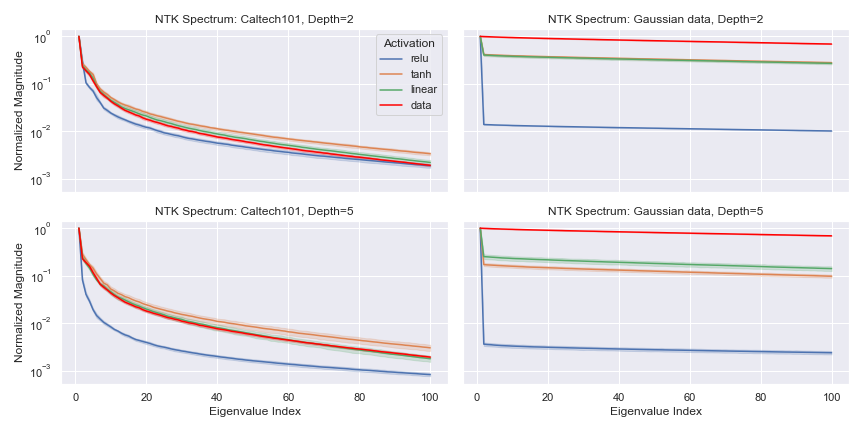
\includegraphics[width=\textwidth]{conference_files/images/cnn_spectrums2.png}
    \caption{\textbf{(NTK Spectrum for CNNs)} We plot the normalized eigenvalues $\lambda_p / \lambda_1$ of the NTK Gram matrix $\mK$ and the data Gram matrix $\mX \mX^T$ for Caltech101 and isotropic Gaussian datasets. To compute the NTK, we randomly initialize convolutional neural networks of depth $2$ and $5$ with $100$ channels per layer. We use the standard parameterization and Pytorch's default Kaiming uniform initialization in order to better connect our results with what is used in practice. We consider a batch size of $n = 200$ and plot the first $100$ eigenvalues. The thick part of each curve corresponds to the mean across 10 trials while the transparent part corresponds to the 95\% confidence interval.}
    \label{fig:spectrum_cnn}
\end{figure}
\begin{figure}[ht]
    \centering    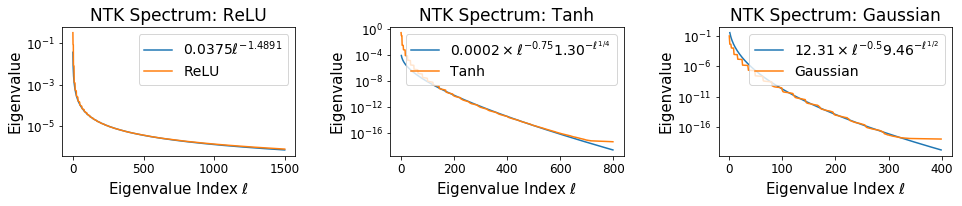
\includegraphics[width=\textwidth]{conference_files/images/asym_spectrum.png}
    \caption{\textbf{ (Asymptotic NTK Spectrum) }NTK spectrum of two-layer fully connected networks with ReLU, Tanh and Gaussian activations under the NTK parameterization. The orange curve is the experimental eigenvalue. The blue curves in the left shows the regression fit for the experimental eigenvalues as a function of eigenvalue index $\ell$ in the form of $\lambda_\ell=a\ell^{-b}$ where $a$ and $b$ are unknown parameters determined by regression. The blue curves in the middle shows the regression fit for the experimental eigenvalues in the form of $\lambda_\ell=a\ell^{-0.75}b^{-l^{1/4}}$. The blue curves in the right shows the regression fit for the experimental eigenvalues in the form of $\lambda_\ell=a\ell^{-0.5}b^{-l^{1/2}}$.}
    \label{fig:asym_spectrum}
\end{figure}
We experimentally test the theory developed in Section \ref{subsec:partial_trace} and its implications by analyzing the spectrum of the NTK for both fully connected neural network architectures (FCNNs), the results of which are displayed in Figure~\ref{fig:spectrum_cifar}, and also convolutional neural network architectures (CNNs), shown in Figure~\ref{fig:spectrum_cnn}. For the feedforward architectures we consider networks of depth 2 and 5 with the width of all layers being set at 500. With regard to the activation function we test linear, ReLU and Tanh, and in terms of initialization we use Kaiming uniform \citep{7410480}, which is very common in practice and is the default in PyTorch \citep{NEURIPS2019_9015}. For the convolutional architectures we again consider depths 2 and 5, with each layer consisting of 100 channels with the filter size set to 5x5. In terms of data, we consider 40x40 patches from both real world images, generated by applying Pytorch's \texttt{RandomResizedCrop} transform to a random batch of Caltech101 images \citep{li_andreeto_ranzato_perona_2022}, as well as synthetic images corresponding to isotropic Gaussian vectors. The batch sized is fixed at 200 and we plot only the first 100 normalized eigenvalues. Each experiment was repeated 10 times. Finally, to compute the NTK we use the \texttt{functorch}\footnote{https://pytorch.org/functorch/stable/notebooks/neural\_tangent\_kernels.html} module in PyTorch using an algorithmic approach inspired by \cite{pmlr-v162-novak22a}. 

The results for convolutional neural networks show the same trends as observed in feedforward neural networks, which we discussed in Section \ref{subsec:partial_trace}. In particular, we again observe the dominant outlier eigenvalue, which increases with both depth and the size of the Gaussian mean of the activation. We also again see that the NTK spectrum inherits its structure from the data, i.e., is skewed for skewed data or relatively flat for isotropic Gaussian data. Finally, we also see that the spectrum for Tanh is closer to the spectrum for the linear activation when compared with the ReLU spectrum. In terms of differences between the CNN and FCNN experiments, we observe that the spread of the 95\% confidence interval is slightly larger for convolutional nets, implying a slightly larger variance between trials. We remark that this is likely attributable to the fact that there are only 100 channels in each layer and by increasing this quantity we would expect the variance to reduce. In summary, despite the fact that our analysis is concerned with FCNNs, it appears that the broad implications and trends also hold for CNNs. We leave a thorough study of the NTK spectrum for CNNs and other network architectures to future work.


To test our theory in Section \ref{subsec:lower}, we numerically plot the spectrum of NTK of two-layer feedforward networks with ReLU, Tanh, and Gaussian activations in Figure~\ref{fig:asym_spectrum}. The input data are uniformly drawn from $\mathbb{S}^2$. Notice that when $d=2$, $k=\Theta(\ell^{1/2})$. Then Corollary~\ref{cor:ReLUbias0} shows that for the ReLU activation $\lambda_\ell=\Theta(\ell^{-3/2})$, for the Tanh activation $\lambda_\ell=O\left(\ell^{-3/4}\exp(-\frac{\pi}{2}\ell^{1/4})\right)$, and for the Gaussian activation $\lambda_\ell=O(\ell^{-1/2}2^{-\ell^{1/2}})$. These theoretical decay rates for the NTK spectrum are verified by the experimental results in Figure~\ref{fig:asym_spectrum}.



\subsection{Analysis of the lower spectrum: uniform data}\label{appendix:lower_uniform}

\unifEigDecay* 

\begin{proof}
Let $\theta(t)=\sum_{p = 0}^{\infty} c_p t^p$, then $K(x_1,x_2)=\theta(\langle x_1, x_2 \rangle)$
According to Funk Hecke theorem \cite[Section 4.2]{uniform_sphere_data}, we have
\begin{align}
    \overline{\lambda_k} = \mathrm{Vol}(\mathbb{S}^{d-1})\int_{-1}^1 \theta(t)P_{k,d}(t)(1-t^2)^{\frac{d-2}{2}}\mathrm{d}t,
    \label{eq:eigenvalue_k}
\end{align}
where $\mathrm{Vol}(\mathbb{S}^{d-1})=\frac{2 \pi^{d/2}}{\Gamma(d/2)}$ is the volume of the hypersphere $\mathbb{S}^{d-1}$, and $P_{k,d}(t)$ is the Gegenbauer polynomial, given by
\begin{equation*}
    P_{k,d}(t)=\frac{(-1)^k}{2^k}\frac{\Gamma(d/2)}{\Gamma(k+d/2)}\frac{1}{(1-t^2)^{(d-2)/2}}\frac{d^k}{dt^k}(1-t^2)^{k+(d-2)/2},
\end{equation*} 
and $\Gamma$ is the gamma function. 

From \eqref{eq:eigenvalue_k} we have
\begin{align}
\overline{\lambda_k} &= \mathrm{Vol}(\mathbb{S}^{d-1})\int_{-1}^1 \theta(t)P_{k,d}(t)(1-t^2)^{\frac{d-2}{2}}\mathrm{d}t \nonumber\\
&= \frac{2\pi^{d/2}}{\Gamma(d/2)}\int_{-1}^1 \theta(t)\frac{(-1)^k}{2^k}\frac{\Gamma(d/2)}{\Gamma(k+d/2)}\frac{d^k}{dt^k}(1-t^2)^{k+(d-2)/2}\mathrm{d}t \nonumber\\
&= \frac{2\pi^{d/2}}{\Gamma(d/2)}\frac{(-1)^k}{2^k}\frac{\Gamma(d/2)}{\Gamma(k+d/2)}\sum_{p=0}^\infty c_p\int_{-1}^1 t^p\frac{d^k}{dt^k}(1-t^2)^{k+(d-2)/2}\mathrm{d}t.
\label{eq:lambda_k_sum}
\end{align}
Using integration by parts, we have
\begin{align}
    &\int_{-1}^1 t^p\frac{d^k}{dt^k}(1-t^2)^{k+(d-2)/2}\mathrm{d}t \nonumber\\
    &=\left. t^p\frac{d^{k-1}}{dt^{k-1}}(1-t^2)^{k+(d-2)/2}\right|_{-1}^1-p\int_{-1}^1 t^{p-1}\frac{d^{k-1}}{dt^{k-1}}(1-t^2)^{k+(d-2)/2}\mathrm{d}t \nonumber\\
    &=-p\int_{-1}^1 t^{p-1}\frac{d^{k-1}}{dt^{k-1}}(1-t^2)^{k+(d-2)/2}\mathrm{d}t,  
    \label{eq:parts_step2}
\end{align}
where the last line in \eqref{eq:parts_step2} holds because $\frac{d^{k-1}}{dt^{k-1}}(1-t^2)^{k+(d-2)/2}=0$ when $t=1$ or $t=-1$.

When $p<k$, repeat the above procedure \eqref{eq:parts_step2} $p$ times, we get
\begin{align}
    \int_{-1}^1 t^p\frac{d^k}{dt^k}(1-t^2)^{k+(d-2)/2}\mathrm{d}t&=(-1)^p p!\int_{-1}^1 \frac{d^{k-p}}{dt^{k-p}}(1-t^2)^{k+(d-2)/2}\mathrm{d}t \nonumber\\
    &=(-1)^p p!\left. \frac{d^{k-p-1}}{dt^{k-p-1}}(1-t^2)^{k+(d-2)/2}\right|_{-1}^1 \nonumber\\
    &=0.
    \label{eq:p<k}
\end{align}
When $p\geq k$, repeat the above procedure \eqref{eq:parts_step2} $k$ times, we get
\begin{align}
    \int_{-1}^1 t^p\frac{d^k}{dt^k}(1-t^2)^{k+(d-2)/2}\mathrm{d}t&=(-1)^k p(p-1)\cdots(p-k+1)\int_{-1}^1 t^{p-k} (1-t^2)^{k+(d-2)/2}\mathrm{d}t.
    \label{eq:r>=k}
\end{align}
When $p-k$ is odd, $t^{p-k} (1-t^2)^{k+(d-2)/2}$ is an odd function, then 
\begin{equation}
    \int_{-1}^1 t^{p-k} (1-t^2)^{k+(d-2)/2}\mathrm{d}t=0.
    \label{eq:odd_case}
\end{equation}
When $p-k$ is even, 
\begin{align}
    \int_{-1}^1 t^{p-k} (1-t^2)^{k+(d-2)/2}\mathrm{d}t&=2\int_{0}^1 t^{p-k} (1-t^2)^{k+(d-2)/2}\mathrm{d}t \nonumber\\
    &=\int_{0}^1 (t^2)^{(p-k-1)/2} (1-t^2)^{k+(d-2)/2}\mathrm{d}t^2 \nonumber\\
    &=B\left(\frac{p-k+1}{2}, k+d/2\right) \nonumber\\
    &=\frac{\Gamma(\frac{p-k+1}{2})\Gamma(k+d/2)}{\Gamma(\frac{p-k+1}{2}+k+d/2)}\label{eq:even_case},
\end{align}
where $B$ is the beta function.

Plugging \eqref{eq:even_case} , \eqref{eq:p<k} and \eqref{eq:odd_case} into \eqref{eq:r>=k}, we get
\begin{align}
    &\int_{-1}^1 t^p\frac{d^k}{dt^k}(1-t^2)^{k+(d-2)/2}\mathrm{d}t \nonumber\\
    &=
    \begin{cases}
    (-1)^k p(p-1)\ldots(p-k+1)\frac{\Gamma(\frac{p-k+1}{2})\Gamma(k+d/2)}{\Gamma(\frac{p-k+1}{2}+k+d/2)}, & p-k \text{ is even and } p\geq k, \\
    0, & \text{otherwise}.
    \end{cases}
    \label{eq:integral_result}
\end{align}
Plugging \eqref{eq:integral_result} into \eqref{eq:lambda_k_sum}, we get
\begin{align*}
\overline{\lambda_k} 
&= \frac{2\pi^{d/2}}{\Gamma(d/2)}\frac{(-1)^k}{2^k}\frac{\Gamma(d/2)}{\Gamma(k+d/2)}\sum_{\substack{p\geq k\\p-k\text{ is even}}} c_p (-1)^k p(p-1)\ldots(p-k+1)\frac{\Gamma(\frac{p-k+1}{2})\Gamma(k+d/2)}{\Gamma(\frac{p-k+1}{2}+k+d/2)}\\
&= \frac{\pi^{d/2}}{2^{k-1}}\sum_{\substack{p\geq k\\p-k\text{ is even}}} c_p \frac{ p(p-1)\ldots(p-k+1)\Gamma(\frac{p-k+1}{2})}{\Gamma(\frac{p-k+1}{2}+k+d/2)}\\
&= \frac{\pi^{d/2}}{2^{k-1}}\sum_{\substack{p\geq k\\p-k\text{ is even}}} c_p \frac{ \Gamma(p+1)\Gamma(\frac{p-k+1}{2})}{\Gamma(p-k+1)\Gamma(\frac{p-k+1}{2}+k+d/2)}.
\end{align*} 
\end{proof} 

\ReLUbiaszero* \label{cor:app:eigendecay} 

\begin{proof}[Proof of Corollary \ref{cor:app:eigendecay}, part 1]
We first prove $\overline{\lambda_k}=O(k^{-d-2a+2})$. Suppose that $c_p\leq C p^{-a}$ for some constant $C$, then according to Theorem~\ref{thm:eigen_hypersphere} we have
\begin{align*}
\overline{\lambda_k} 
&\leq \frac{\pi^{d/2}}{2^{k-1}}\sum_{\substack{p\geq k\\p-k\text{ is even}}} C p^{-a} \frac{ \Gamma(p+1)\Gamma(\frac{p-k+1}{2})}{\Gamma(p-k+1)\Gamma(\frac{p-k+1}{2}+k+d/2)}.
\end{align*}
According to Stirling's formula, we have
\begin{equation}
\label{eq:stirling}
    \Gamma(z)=\sqrt{\frac{2\pi}{z}}\left(\frac{z}{e}\right)^z\left(1+O\left(\frac{1}{z}\right)\right).
\end{equation}
Then for any $z\geq \frac{1}{2}$, we can find constants $C_1$ and $C_2$ such that
\begin{equation}
\label{eq:stirling_1}
    C_1\sqrt{\frac{2\pi}{z}}\left(\frac{z}{e}\right)^z\leq\Gamma(z)\leq C_2\sqrt{\frac{2\pi}{z}}\left(\frac{z}{e}\right)^z.
\end{equation}
Then 
\begin{align}
\overline{\lambda_k} 
&\leq \frac{\pi^{d/2}}{2^{k-1}}\frac{C_2^2}{C_1^2}\sum_{\substack{p\geq k\\p-k\text{ is even}}} C p^{-a} \frac{ \sqrt{\frac{2\pi}{p+1}}\left(\frac{p+1}{e}\right)^{p+1}\sqrt{\frac{2\pi}{\frac{p-k+1}{2}}}\left(\frac{\frac{p-k+1}{2}}{e}\right)^\frac{p-k+1}{2}}{\sqrt{\frac{2\pi}{{p-k+1}}}\left(\frac{p-k+1}{e}\right)^{p-k+1}\sqrt{\frac{2\pi}{\frac{p-k+1}{2}+k+d/2}}\left(\frac{\frac{p-k+1}{2}+k+d/2}{e}\right)^{\frac{p-k+1}{2}+k+d/2}} \nonumber\\
&= \frac{\pi^{d/2}}{2^{k-1}}\frac{C_2^2C}{C_1^2}\sum_{\substack{p\geq k\\p-k\text{ is even}}}p^{-a} \frac{e^{\frac{d}{2}} \sqrt{\frac{2}{p+1}}\left({p+1}\right)^{p+1}\left({\frac{p-k+1}{2}}\right)^\frac{p-k+1}{2}}{\left({p-k+1}\right)^{p-k+1}\sqrt{\frac{1}{\frac{p-k+1}{2}+k+d/2}}\left({\frac{p-k+1}{2}+k+d/2}\right)^{\frac{p-k+1}{2}+k+d/2}} \nonumber\\
&= \frac{\pi^{d/2}}{2^{k-1}}\frac{C_2^2C}{C_1^2}\sum_{\substack{p\geq k\\p-k\text{ is even}}}p^{-a} \frac{e^{\frac{d}{2}}2^{\frac{-p+k}{2}} \left({p+1}\right)^{p+\frac{1}{2}}}{\left({p-k+1}\right)^{\frac{p-k+1}{2}}\left({\frac{p-k+1}{2}+k+d/2}\right)^{\frac{p-k}{2}+k+d/2}} \nonumber\\
&= 2\pi^{d/2}\frac{2^{\frac{d}{2}}e^{\frac{d}{2}}C_2^2C}{C_1^2}\sum_{\substack{p\geq k\\p-k\text{ is even}}} \frac{ p^{-a}\left({p+1}\right)^{p+\frac{1}{2}}}{\left({p-k+1}\right)^{\frac{p-k+1}{2}}\left({p+k+1+d}\right)^{\frac{p+k+d}{2}}}.
\label{eq:lambda_leq}
\end{align}
We define 
\begin{equation}
f_a(p)=\frac{ p^{-a}\left({p+1}\right)^{p+\frac{1}{2}}}{\left({p-k+1}\right)^{\frac{p-k+1}{2}}\left({p+k+1+d}\right)^{\frac{p+k+d}{2}}}. 
\label{eq:def_f}
\end{equation}
By applying the chain rule to $e^{\log f_a(p)}$, we have that the derivative of $f_a$ is
\begin{multline}
f_a'(p)= \frac{(p + 1)^{p + \frac{1}{2}} p^{-a} }{2(p-k+1)^{\frac{p -k+ 1}{2}} (p+k+d+1)^{\frac{p+k+d}{2} }}  \\ \cdot \left(-\frac{2a}{p}   - \frac{k+d}{(p + 1)(p+k+d+1)}  +  \log(1+\frac{k^2-d(p-k+1)}{(p-k+1)(p+k+d+1)})\right).    
\end{multline}
Let $g_a(p)=-\frac{2a}{p}   - \frac{k+d}{(p + 1)(p+k+d+1)}  +  \log(1+\frac{k^2-d(p-k+1)}{(p-k+1)(p+k+d+1)})$. Then $g_a(p)$ and $f_a'(p)$ have the same sign.
Next we will show that $g_a(p)\geq 0$ for $k\leq p\leq  \frac{k^2}{d+24a}$ when $k$ is large enough.

First when $p\geq k$ and 
$\frac{k^2-d(p-k+1)}{(p-k+1)(p+k+d+1)}\geq 1$, we have
\begin{align}
    g_a(p)\geq -\frac{2a}{k}   - \frac{k+d}{(k + 1)(k+k+d+1)}+\log(2) \geq 0,
\end{align}
when $k$ is sufficiently large.

Second when $p\geq k$ and 
$0\leq \frac{k^2-d(p-k+1)}{(p-k+1)(p+k+d+1)}\leq 1$, since $\log(1+x)\geq \frac{x}{2}$ for $0\leq x\leq 1$, we have
\begin{align*}
    g_a(p)&\geq -\frac{2a}{p}   - \frac{k+d}{(p + 1)(p+k+d+1)}+\frac{k^2-d(p-k+1)}{2(p-k+1)(p+k+d+1)}\\
    &\geq -\frac{2a}{p}   - \frac{k+d}{(p + 1)(p+k+d+1)}+\frac{k^2-dp}{2p(p+k+d+1)}.
\end{align*} 
When $p\leq \frac{k^2}{d+24a}$, we have $k^2-dp\geq 24ap$. Then 
\begin{equation*}
   \frac{k^2-dp}{4p(p+k+d+1)}\geq \frac{24ap}{4p(p+k+d+1)}\geq \frac{6ap}{(p+1)(p+k+d+1)} \geq \frac{k+d}{(p + 1)(p+k+d+1)}
\end{equation*} 
when $k$ is sufficiently large. 
Also we have 
\begin{equation*}
   \frac{k^2-dp}{4r(p+k+d+1)}\geq \frac{24ap}{4r(p+k+d+1)}\geq \frac{6a}{p+k+d+1} \geq \frac{2a}{p}
\end{equation*} 
when $k$ is sufficiently large. 

Combining all the arguments above, we conclude that $g_a(p)\geq 0$ and $f_a'(p)\geq 0$ when $k\leq p \leq \frac{k^2}{d+24a}$. 
Then when $k\leq p \leq \frac{k^2}{d+24a}$, we have 
\begin{equation}
    f_a(p)\leq f_a\left(\frac{k^2}{d+24a}\right).
    \label{eq:fa_small_p}
\end{equation} 
When $p \geq \frac{k^2}{d+24a}$, we have 
\begin{align*}
    f_a(p)&=\frac{ p^{-a}\left({p+1}\right)^{p+\frac{1}{2}}}{\left({p-k+1}\right)^{\frac{p-k+1}{2}}\left({p+k+1+d}\right)^{\frac{p+k+d}{2}}}\\
    &=\frac{ p^{-a}\left({p+1}\right)^{p+\frac{1}{2}}}{\left((p+1)^2-k^2+d(p-k+1)\right)^{\frac{p-k+1}{2}}\left({p+k+1+d}\right)^{\frac{2k+d-1}{2}}}\\
    &=\frac{ p^{-a}\left({p+1}\right)^{-\frac{d}{2}}}{\left(1-\frac{k^2-d(p-k+1)}{(p+1)^2}\right)^{\frac{p-k+1}{2}}\left({1+\frac{k+d}{p+1}}\right)^{\frac{2k+d-1}{2}}}\\
    &\leq\frac{ p^{-a-\frac{d}{2}}}{\left(1-\frac{k^2-d(p-k+1)}{(p+1)^2}\right)^{\frac{p-k+1}{2}}}.
\end{align*} 
If $k^2-d(p-k+1)<0$, $\left(1-\frac{k^2-d(p-k+1)}{(p+1)^2}\right)^{\frac{p-k+1}{2}}\geq 1$. If $k^2-d(p-k+1)\geq 0$, i.e., $p\leq \frac{k^2+dk-d}{d}$, for sufficiently large $k$, we have
\begin{align*}
    \left(1-\frac{k^2-d(p-k+1)}{(p+1)^2}\right)^{\frac{p-k+1}{2}}&\geq\left(1-\frac{k^2-d(\frac{k^2}{d+24a}-k+1)}{(\frac{k^2}{d+24a}+1)^2}\right)^{\frac{\frac{k^2+dk-d}{d}-k+1}{2}}\\
    &\geq \left(1-\frac{48a(d+24a)}{k^2}\right)^{\frac{k^2}{2d}}\\
    &\geq e^{-\frac{k^2}{2d}\frac{48a(d+24a)}{k^2}}= e^{-\frac{48a(d+24a)}{2d}},
\end{align*}
which is a constant independent of $k$. 
Then for $p \geq \frac{k^2}{d+24a}$, we have
\begin{equation}
f_a(p)\leq e^{\frac{48a(d+24a)}{2d}}p^{-a-\frac{d}{2}}.
\label{eq:fa_large_p}
\end{equation}

Finally we have
\begin{align*}
\overline{\lambda_k}&= 2\pi^{d/2}\frac{2^{\frac{d}{2}}e^{\frac{d}{2}}C_2^2C}{C_1^2}\sum_{\substack{p\geq k\\p-k\text{ is even}}} f_a(p)\\
&\leq O\left(\sum_{\substack{k\leq p \leq \frac{k^2}{d+24a}\\p-k\text{ is even}}} f_a(p)+\sum_{\substack{p\geq \frac{k^2}{d+24a}\\p-k\text{ is even}}} f_a(p)\right)\\
&\leq O\left(\left(\frac{k^2}{d+24a}-k+1\right)f_a\left(\frac{k^2}{d+24a}\right)+\sum_{\substack{p\geq \frac{k^2}{d+24a}\\p-k\text{ is even}}} e^{\frac{48a(d+24a)}{2d}}p^{-a-\frac{d}{2}}\right)\\
&\leq O\left(\left(\frac{k^2}{d+24a}-k+1\right)e^{\frac{48a(d+24a)}{2d}}\left(\frac{k^2}{d+24a}\right)^{-a-\frac{d}{2}}+ e^{\frac{48a(d+24a)}{2d}}\frac{1}{{a+\frac{d}{2}-1}}\left(\frac{k^2}{d+24a}-1\right)^{1-a-\frac{d}{2}}\right)\\
&=O(k^{-d-2a+2}).
\end{align*} 

Next we prove $\overline{\lambda_k}=\Omega(k^{-d-2a+2})$. Since $c_p$ are nonnegative and $c_p=\Theta(p^{-a})$, we have that $c_p\geq C' p^{-a}$ for some constant $C'$. Then we have
\begin{align}
\overline{\lambda_k} 
&\geq \frac{\pi^{d/2}}{2^{k-1}}\sum_{\substack{p\geq k\\p-k\text{ is even}}} C' p^{-a} \frac{ \Gamma(p+1)\Gamma(\frac{p-k+1}{2})}{\Gamma(p-k+1)\Gamma(\frac{p-k+1}{2}+k+d/2)}.
\end{align} 
According to Stirling's formula \eqref{eq:stirling} and \eqref{eq:stirling_1}, using the similar argument as \eqref{eq:lambda_leq} we have
\begin{align}
\overline{\lambda_k} 
&\geq \frac{\pi^{d/2}}{2^{k-1}}\frac{C_1^2}{C_2^2}\sum_{\substack{p\geq k\\p-k\text{ is even}}} C' p^{-a} \frac{ \sqrt{\frac{2\pi}{p+1}}\left(\frac{p+1}{e}\right)^{p+1}\sqrt{\frac{2\pi}{\frac{p-k+1}{2}}}\left(\frac{\frac{p-k+1}{2}}{e}\right)^\frac{p-k+1}{2}}{\sqrt{\frac{2\pi}{{p-k+1}}}\left(\frac{p-k+1}{e}\right)^{p-k+1}\sqrt{\frac{2\pi}{\frac{p-k+1}{2}+k+d/2}}\left(\frac{\frac{p-k+1}{2}+k+d/2}{e}\right)^{\frac{p-k+1}{2}+k+d/2}}\\
\label{eq:lambda_geq}
&= 2\pi^{d/2}\frac{2^{\frac{d}{2}}e^{\frac{d}{2}}C_1^2C'}{C_2^2}\sum_{\substack{p\geq k\\p-k\text{ is even}}} \frac{ p^{-a}\left({p+1}\right)^{p+\frac{1}{2}}}{\left({p-k+1}\right)^{\frac{p-k+1}{2}}\left({p+k+1+d}\right)^{\frac{p+k+d}{2}}}\\
&\geq 2\pi^{d/2}\frac{2^{\frac{d}{2}}e^{\frac{d}{2}}C_1^2C'}{C_2^2}\sum_{\substack{p\geq k^2\\p-k\text{ is even}}} f_a(p),
\end{align}
where $f_a(p)$ is defined in \eqref{eq:def_f}. 
When $p \geq k^2$, we have
\begin{align*}
    f_a(p)&=\frac{ p^{-a}\left({p+1}\right)^{p+\frac{1}{2}}}{\left({p-k+1}\right)^{\frac{p-k+1}{2}}\left({p+k+1+d}\right)^{\frac{p+k+d}{2}}}\\
    &=\frac{ p^{-a}\left({p+1}\right)^{p+\frac{1}{2}}}{\left((p+1)^2-k^2+d(p-k+1)\right)^{\frac{p-k+1}{2}}\left({p+k+1+d}\right)^{\frac{2k+d-1}{2}}}\\
    &\geq\frac{ \left({p+1}\right)^{-a-\frac{d}{2}}}{\left(1-\frac{k^2-d(p-k+1)}{(p+1)^2}\right)^{\frac{p-k+1}{2}}\left({1+\frac{k+d}{p+1}}\right)^{\frac{2k+d-1}{2}}}
\end{align*}
For sufficiently large $k$, $k^2-d(p-k+1)<0$. Then we have
\begin{align*}
    \left(1-\frac{k^2-d(p-k+1)}{(p+1)^2}\right)^{\frac{p-k+1}{2}}&= \left(1-\frac{k^2-d(p-k+1)}{(p+1)^2}\right)^{\frac{-(p+1)^2}{k^2-d(p-k+1)}\cdot\frac{-k^2+d(p-k+1)}{(p+1)^2}\cdot\frac{p-k+1}{2}}\\
    &\leq e^{\frac{-k^2+d(p-k+1)}{(p+1)^2}\cdot\frac{p-k+1}{2}}\\
    &\leq e^{\frac{dp^2}{2p^2}}=e^{\frac{d}{2}}
\end{align*} 
which is a constant independent of $k$. 
Also, for sufficiently large $k$, we have 
\begin{align*}
    \left({1+\frac{k+d}{p+1}}\right)^{\frac{2k+d-1}{2}}&= \left({1+\frac{k+d}{p+1}}\right)^{\frac{p+1}{k+d}\frac{k+d}{p+1}\frac{2k+d-1}{2}}\\
    &\leq e^{\frac{k+d}{p+1}\frac{2k+d-1}{2}}\\
    &\leq e^{\frac{3k^2}{2r}}=e^{\frac{3}{2}}
\end{align*}

Then for $p \geq k^2$, we have $f_a(p)\geq e^{-\frac{d}{2}-\frac{3}{2}}(p+1)^{-a-\frac{d}{2}}$.

Finally we have 
\begin{align}
\overline{\lambda_k} 
&\geq 2\pi^{d/2}\frac{2^{\frac{d}{2}}e^{\frac{d}{2}}C_1^2C'}{C_2^2}\sum_{\substack{p\geq k^2\\p-k\text{ is even}}} f_a(p)\\
&\geq 2\pi^{d/2}\frac{2^{\frac{d}{2}}e^{\frac{d}{2}}C_1^2C'}{C_2^2}\sum_{\substack{p\geq k^2\\p-k\text{ is even}}} e^{-\frac{d}{2}-\frac{3}{2}}(p+1)^{-a-\frac{d}{2}}\\
&\geq 2\pi^{d/2}\frac{2^{\frac{d}{2}}e^{\frac{d}{2}}C_1^2C'}{C_2^2} e^{-\frac{d}{2}-\frac{3}{2}}\frac{1}{2(a+\frac{d}{2}-1)}(k^2+2)^{1-a-\frac{d}{2}}\\
&=\Omega(k^{-d-2a+2}).
\end{align}
Overall, we have $\overline{\lambda_k} =\Theta(k^{-d-2a+2})$.
\end{proof}
\begin{proof}[Proof of Corollary \ref{cor:app:eigendecay}, part 2]
It is easy to verify that $\overline{\lambda_k}=0$ when $k$ is even because $c_p=0$ when $p\geq k$ and $p-k$ is even. When $k$ is odd, the proof of Theorem~\ref{thm:eigen_hypersphere} still applies.
\end{proof}

\begin{proof}[Proof of Corollary \ref{cor:app:eigendecay}, part 3]
Since $c_p = \cO\left(\exp\left( - a\sqrt{p}\right) \right)$, 
 we have that $c_p\leq C e^{-a\sqrt{p}}$ for some constant $C$. 
Similar to \eqref{eq:lambda_leq}, we have
\begin{align}
\overline{\lambda_k} 
&\leq 2\pi^{d/2}\frac{2^{\frac{d}{2}}e^{\frac{d}{2}}C_2^2C}{C_1^2}\sum_{\substack{p\geq k\\p-k\text{ is even}}} \frac{  e^{-a\sqrt{p}}\left({p+1}\right)^{p+\frac{1}{2}}}{\left({p-k+1}\right)^{\frac{p-k+1}{2}}\left({p+k+1+d}\right)^{\frac{p+k+d}{2}}}.
\end{align}
Use the definition in \eqref{eq:def_f} and let $a=0$, we have
\begin{equation}
f_0(p)=\frac{\left({p+1}\right)^{p+\frac{1}{2}}}{\left({p-k+1}\right)^{\frac{p-k+1}{2}}\left({p+k+1+d}\right)^{\frac{p+k+d}{2}}}. 
\end{equation}
Then according to \eqref{eq:fa_small_p} and \eqref{eq:fa_large_p}, for sufficiently large $k$, we have $f_0(p)\leq f_0\left(\frac{k^2}{d}\right)$ when $k\leq p \leq \frac{k^2}{d}$ and $f_0(p)\leq C_3p^{-\frac{d}{2}}$ for some constant $C_3$ when $p\geq \frac{k^2}{d}$. Then when $k\leq p \leq \frac{k^2}{d}$, we have $f_0(p)\leq f_0\left(\frac{k^2}{d}\right)\leq C_3 \left(\frac{k^2}{d}\right)^{-\frac{d}{2}}$. When $p\geq \frac{k^2}{d}$, we have $f_0(p)\leq C_3p^{-\frac{d}{2}}\leq C_3\left(\frac{k^2}{d}\right)^{-\frac{d}{2}}$. Overall, for all $p\geq k$, we have
\begin{equation}
f_0(p)\leq  C_3\left(\frac{k^2}{d}\right)^{-\frac{d}{2}}.
\end{equation}
Then we have 
\begin{align}
\overline{\lambda_k} 
&\leq 2\pi^{d/2}\frac{2^{\frac{d}{2}}e^{\frac{d}{2}}C_2^2C}{C_1^2}\sum_{\substack{p\geq k\\p-k\text{ is even}}} e^{-a\sqrt{p}}f_0(p)\\
&\leq 2\pi^{d/2}\frac{2^{\frac{d}{2}}e^{\frac{d}{2}}C_2^2C_3C}{C_1^2}\left(\frac{k^2}{d}\right)^{-\frac{d}{2}}\sum_{\substack{p\geq k\\p-k\text{ is even}}} e^{-a\sqrt{p}}\\
&\leq 2\pi^{d/2}\frac{2^{\frac{d}{2}}e^{\frac{d}{2}}C_2^2C_3C}{C_1^2}\left(\frac{k^2}{d}\right)^{-\frac{d}{2}}\frac{2e^{-a\sqrt{k-1}}(a\sqrt{k-1}+1)}{a^2}\\
&=\cO\left(k^{-d+1/2}\exp\left( - a\sqrt{k}\right) \right)
\end{align}
\end{proof}

\begin{proof}[Proof of Corollary \ref{cor:app:eigendecay}, part 4]
Since $c_p = \Theta(p^{1/2} a^{-p})$, 
 we have that $c_p\leq C p^{1/2} a^{-p}$ for some constant $C$. 
Similar to \eqref{eq:lambda_leq}, we have
\begin{align}
\overline{\lambda_k} 
&\leq 2\pi^{d/2}\frac{2^{\frac{d}{2}}e^{\frac{d}{2}}C_2^2C}{C_1^2}\sum_{\substack{p\geq k\\p-k\text{ is even}}} \frac{  p^{1/2} a^{-p}\left({p+1}\right)^{p+\frac{1}{2}}}{\left({p-k+1}\right)^{\frac{p-k+1}{2}}\left({p+k+1+d}\right)^{\frac{p+k+d}{2}}}.
\end{align}
Use the definition in \eqref{eq:def_f} and let $a=0$, we have
\begin{equation}
f_0(p)=\frac{\left({p+1}\right)^{p+\frac{1}{2}}}{\left({p-k+1}\right)^{\frac{p-k+1}{2}}\left({p+k+1+d}\right)^{\frac{p+k+d}{2}}}. 
\end{equation}
Then according to \eqref{eq:fa_small_p} and \eqref{eq:fa_large_p}, for sufficiently large $k$, we have $f_0(p)\leq f_0\left(\frac{k^2}{d}\right)$ when $k\leq p \leq \frac{k^2}{d}$ and $f_0(p)\leq C_3p^{-\frac{d}{2}}$ for some constant $C_3$ when $p\geq \frac{k^2}{d}$. Then when $k\leq p \leq \frac{k^2}{d}$, we have $p^{1/2}f_0(p)\leq p^{1/2} f_0\left(\frac{k^2}{d}\right)\leq C_3 \left(\frac{k^2}{d}\right)^{1/2} \left(\frac{k^2}{d}\right)^{-\frac{d}{2}}$. When $p\geq \frac{k^2}{d}$, we have $p^{1/2}f_0(p)\leq C_3 p^{1/2}p^{-\frac{d}{2}}\leq C_3\left(\frac{k^2}{d}\right)^{-\frac{d}{2}+\frac{1}{2}}$. Overall, for all $p\geq k$, we have
\begin{equation}
p^{1/2}f_0(p)\leq  C_3 \left(\frac{k^2}{d}\right)^{-\frac{d}{2}+\frac{1}{2}}.
\end{equation}
Then we have 
\begin{align}
\overline{\lambda_k} 
&\leq 2\pi^{d/2}\frac{2^{\frac{d}{2}}e^{\frac{d}{2}}C_2^2C}{C_1^2}\sum_{\substack{p\geq k\\p-k\text{ is even}}} p^{1/2} a^{-p}f_0(p)\\
&\leq 2\pi^{d/2}\frac{2^{\frac{d}{2}}e^{\frac{d}{2}}C_2^2C_3C}{C_1^2}\left(\frac{k^2}{d}\right)^{-\frac{d}{2}+\frac{1}{2}}\sum_{\substack{p\geq k\\p-k\text{ is even}}}  a^{-p}\\
&\leq 2\pi^{d/2}\frac{2^{\frac{d}{2}}e^{\frac{d}{2}}C_2^2C_3C}{C_1^2}\left(\frac{k^2}{d}\right)^{-\frac{d}{2}+\frac{1}{2}}\frac{1}{\log a}a^{-(k-1)}\\
&=\cO\left(k^{-d+1}a^{-k} \right).
\end{align}
On the other hand, since $c_p = \Theta(p^{1/2} a^{-p})$, we have that $c_p\geq C' p^{1/2} a^{-p}$ for some constant $C'$. Similar to \eqref{eq:lambda_geq}, we have
\begin{align}
\overline{\lambda_k} 
&\geq 2\pi^{d/2}\frac{2^{\frac{d}{2}}e^{\frac{d}{2}}C_1^2C'}{C_2^2}\sum_{\substack{p\geq k\\p-k\text{ is even}}} \frac{  p^{1/2} a^{-p}\left({p+1}\right)^{p+\frac{1}{2}}}{\left({p-k+1}\right)^{\frac{p-k+1}{2}}\left({p+k+1+d}\right)^{\frac{p+k+d}{2}}}\\
&\geq 2\pi^{d/2}\frac{2^{\frac{d}{2}}e^{\frac{d}{2}}C_1^2C'}{C_2^2}\frac{  k^{1/2} a^{-k}\left({k+1}\right)^{k+\frac{1}{2}}}{\left({k-k+1}\right)^{\frac{k-k+1}{2}}\left({k+k+1+d}\right)^{\frac{k+k+d}{2}}}\\
&=\Omega\left(\frac{  k^{-d/2+1} a^{-k}\left({k+1}\right)^{k}}{\left({k+k+1+d}\right)^{k}}\right).
\end{align}
Since $\left({k+1}\right)^{k}=k^k(1+1/k)^k=\Theta(k^k)$. Similarly, $\left({k+k+1+d}\right)^{k}=\Theta((2k)^k)$. Then we have
\begin{align}
\overline{\lambda_k} 
&=\Omega\left(\frac{  k^{-d/2+1} a^{-k}\left({k+1}\right)^{k}}{\left({k+k+1+d}\right)^{k}}\right)\\
&=\Omega\left(\frac{  k^{-d/2+1} a^{-k}k^k}{(2k)^{k}}\right)\\
&=\Omega\left(  k^{-d/2+1}2^{-k} a^{-k}\right).
\end{align}
\end{proof}

For the NTK of a two-layer ReLU network with $\gamma_b>0$, then according to Lemma~\ref{lemma:ntk_2layer_coeff_decay} we have  $c_p=\kappa_{p,2}=\Theta(p^{-3/2})$ . 
Therefore using Corollary~\ref{cor:ReLUbias0} $\overline{\lambda_k} = \Theta(k^{-d-1})$. 
Notice here that $k$ refers to the frequency, and the number of spherical harmonics of frequency at most $ k$ is $\Theta(k^d)$. 
Therefore, for the $\ell$th largest eigenvalue $\lambda_\ell$ we have $\lambda_\ell=\Theta(\ell^{-(d+1)/d})$. 
This rate agrees with \cite{uniform_sphere_data} and \cite{NEURIPS2021_14faf969}. 
 For the NTK of a two-layer ReLU network with $\gamma_b=0$, the eigenvalues corresponding to the even frequencies are $0$, which also agrees with \cite{uniform_sphere_data}. 
Corollary~\ref{cor:ReLUbias0} also shows the decay rates of eigenvalues for the NTK of two-layer networks with Tanh activation and Gaussian activation.  We observe that when the coefficients of the kernel power series decay quickly then the eigenvalues of the kernel also decay quickly. As a faster decay of the eigenvalues of the kernel implies a smaller RKHS, Corollary \ref{cor:ReLUbias0} demonstrates that using ReLU results in a larger RKHS relative to using either Tanh or Gaussian activations. We numerically illustrate Corollary \ref{cor:ReLUbias0} in Figure~\ref{fig:asym_spectrum}, Appendix~\ref{appendix:subsection:emp_validation_ef}.

\subsection{Analysis of the lower spectrum: non-uniform data}\label{appendix:lower_non_uniform}
The purpose of this section is to prove a formal version of Theorem \ref{theorem:informal_ub_eigs_nonuniform}. In order to prove this result we first need the following lemma.

\begin{lemma}\label{lemma:eigen_ub_nonuniform1}
     Let the coefficients $(c_j)_{j=0}^\infty$ with $c_j \in \reals_{\geq 0}$ for all $j \in \ints_{\geq 0}$ be such that the series $\sum_{j=0}^{\infty} c_j \rho^j$ converges for all $\rho \in [-1,1]$. Given a data matrix $\mX \in \reals^{n \times d}$ with $\norm{\vx_i} = 1$ for all $i \in [n]$, define $r \defeq \operatorname{rank}(\mX) \geq 2$ and the gram matrix $\mG\defeq \mX \mX^T$. Consider the kernel matrix
    \[
        n\mK = \sum_{j=0}^{\infty}c_j \mG^{\odot j} . 
    \]
    For arbitrary $m \in \ints_{\geq 1}$, let the eigenvalue index $k$ satisfy $n \geq k > \operatorname{rank} \left( \mH_m \right)$, where $\mH_m \defeq \sum_{j=0}^{m-1} c_j \mG^{\odot j}$. Then
    \begin{equation} \label{eq:eig_ub1_nonuniform}
        \lambda_k(\mK) \leq \frac{\norm{\mG^{\odot m}}}{n} \sum_{j=m}^{\infty} c_j.
    \end{equation}
\end{lemma}
\begin{proof}
    We start our analysis by considering $\lambda_k(n\mK)$ for some arbitrary $k \in \naturals_{\leq n}$. Let
    \[
    \begin{aligned}
    \mH_m &\defeq  \sum_{j=0}^{m-1} c_j \mG^{\odot j},\\
    \mT_m &\defeq \sum_{j=m}^{\infty} c_j \mG^{\odot j}
    \end{aligned}
    \]
    be the $m$-head and $m$-tail of the Hermite expansion of $n\mK$: clearly $n\mK = \mH_m + \mT_m$ for any $m \in \naturals$.  Recall that a constant matrix is symmetric and positive semi-definite, furthermore, by the Schur product theorem, the Hadamard product of two positive semi-definite matrices is positive semi-definite.  As a result, $\mG^{\odot j}$ is symmetric and positive semi-definite for all $j \in \ints_{\geq 0}$ and therefore $\mH_m$ and $\mT_m$ are also symmetric positive semi-definite matrices. 
    From Weyl's inequality \cite[Satz~1]{Weyl} it follows that
    \begin{equation}\label{eq:weyl}
        n\lambda_k(\mK) \leq \lambda_k(\mH_m) + \lambda_1(\mT_m) . 
    \end{equation}
    In order to upper bound $\lambda_1(\mT_m)$, observe, as $\mT_m$ is square, symmetric and positive semi-definite, that $\lambda_1(\mT_m) = \norm{\mT_m}$.  Using the non-negativity of the coefficients $(c_j)_{j=0}^{\infty}$ and the triangle inequality we have
    \[
    \begin{aligned}
    \lambda_1(\mT_m)
     =\norm{\sum_{j=m}^{\infty} c_j \mG^{\odot j}} \leq \sum_{j=m}^{\infty} c_j \norm{\mG^{\odot j}}
    \end{aligned}
    \]
    By the assumptions of the lemma $[\mG]_{ii} = 1$ and therefore $[\mG]_{ii}^j = 1$ for all $j \in \ints_{\geq 0}$. Furthermore, for any pair of positive semi-definite matrices $\mA, \mB \in \reals^{n \times n}$ and $k \in [n]$ 
    \begin{equation}
    \lambda_{1}(\mA \odot \mB) \leq \max_{i \in [n]} [\mA]_{ii} \lambda_{1}(\mB),
    \end{equation}
    \cite{Schur1911}. Therefore, as $\max_{i \in [n]} [\mG]_{ii} = 1$,
    \[
    \norm{\mG^{\odot j}} = \lambda_1(\mG^{\odot j}) = \lambda_1(\mG \odot \mG^{\odot (j-1)}) \leq \lambda_1(\mG^{\odot (j-1)}) = \norm{\mG^{\odot (j-1)}}
    \]
    for all $j \in \naturals$. As a result
    \[
    \begin{aligned}
    \lambda_1(\mT_m) \leq \norm{\mG^{\odot m}} \sum_{j=m}^{\infty} c_j.
    \end{aligned}
    \]
    Finally, we now turn our attention to the analysis of $\lambda_k(\mH_m)$. Upper bounding a small eigenvalue is typically challenging, however, the problem simplifies when and $k$ exceeds the rank of $\mH_m$, as is assumed here, as this trivially implies $\lambda_k(\mH_m) = 0$. Therefore, for $k > \operatorname{rank}(\mH_m)$
    \[
    \lambda_k(\mK) \leq \frac{\norm{\mG^m}}{n} \sum_{j=m}^{\infty} c_j 
    \]
    as claimed.
\end{proof}

In order to use Lemma \ref{lemma:eigen_ub_nonuniform1} we require an upper bound on the rank of $\mH_m$. To this end we provide Lemma \ref{lemma:rankH}.

\begin{lemma}\label{lemma:rankH}
     Let $\mG\in \reals^{n \times n}$ be a symmetric, positive semi-definite matrix of rank $2 \leq r \leq d$. Define $\mH_m \in \reals^{n \times n}$ as 
     \begin{equation}
         \mH_m = \sum_{j=0}^{m-1} c_j \mG^{\odot j}
     \end{equation}
     where $(c_j)_{j=0}^{m-1}$ is a sequence of real coefficients. Then
     \begin{equation}
     \begin{aligned}
         \text{rank}\left(\mH_m \right) \leq &1 + \min\{r-1, m-1 \}(2e)^{r-1} \\
         &+ \max\{0, m-r\}\left(\frac{2e}{r-1}\right)^{r-1} (m-1)^{r-1}.
         \end{aligned}
     \end{equation}
\end{lemma}


\begin{proof}
    As $\mG$ is a symmetric and positive semi-definite matrix, its eigenvalues are real and non-negative and its eigenvectors are orthogonal. Let $\{ \vv_i \}_{i=1}^r$ be a set of orthogonal eigenvectors for $\mG$ and $\gamma_i$ the eigenvalue associated with $\vv_i\in \reals^n$. Then $\mG$ may be written as a sum of rank one matrices as follows,
    \[
    \mG = \sum_{i=1}^{r} \gamma_i \vv_i \vv_i^T.
    \]
    As the Hadamard product is commutative, associative and distributive over addition, for any $j\in \ints_{\geq 0}$  $\mG^{\odot j}$ can also be expressed as a sum of rank 1 matrices,
    \[
    \begin{aligned}
    \mG^{\odot j} &= \left(\sum_{i=1}^{r} \gamma_i \vv_i \vv_i^T\right)^{\odot j}\\
    & =  \left(\sum_{i_1=1}^{r} \gamma_{i_1} \vv_{i_1} \vv_{i_1}^T\right) \odot \left(\sum_{i_2=1}^{r} \gamma_{i_2} \vv_{i_2} \vv_{i_2}^T\right) \odot \cdots \odot\left(\sum_{i_j=1}^{r} \gamma_{i_j} \vv_{i_j} \vv_{i_j}^T\right)\\
    & = \sum_{i_1,i_2...i_j=1}^{r} \gamma_{i_1} \gamma_{i_2}\cdots \gamma_{i_r} \left( \vv_{i_1} \vv_{i_1}^T\right) \odot \left( \vv_{i_2} \vv_{i_2}^T\right)\odot\cdots\odot \left(\vv_{i_j} \vv_{i_j}^T \right)\\
    & = \sum_{i_1,i_2,\ldots, i_j=1}^{r} \gamma_{i_1} \gamma_{i_2}\cdots \gamma_{i_j} \left( \vv_{i_1} \odot \vv_{i_2}\odot\cdots \odot \vv_{i_j}\right)\left( \vv_{i_1} \odot \vv_{i_2}\odot\cdots \odot \vv_{i_j}\right)^T.
    \end{aligned}
    \]
    Note the fourth equality in the above follows from $\vv_i \vv_i^T = \vv_i \otimes \vv_i$ and an application of the mixed-product property of the Hadamard product. As matrix rank is sub-additive, the rank of $\mG^{\odot j}$ is less than or equal to the number of distinct rank-one matrix summands. This quantity in turn is equal to the number of vectors of the form $\left( \vv_{i_1} \odot \vv_{i_2}\odot\cdots\odot \vv_{i_j}\right)$, where $i_1, i_2,\ldots, i_j \in [r]$. This in turn is equivalent to computing the number of $j$-combinations with repetition from $r$ objects. 
    Via a stars and bars argument this is equal to $\binom{r+j-1}{j} = \binom{r+j-1}{r(n)-1}$. It therefore follows that
    \[
    \begin{aligned}
    \operatorname{rank}(\mG^{\odot j}) &\leq \binom{r+j-1}{r-1}\\
    & \leq \left(\frac{e(r+j-1)}{r-1} \right)^{r-1}\\
    & \leq  e^{r-1} \left(1 + \frac{j}{r-1} \right)^{r-1}\\
    & \leq (2e)^{r-1} \left(\delta_{j\leq r-1}  + \delta_{j > r-1} \left(\frac{j}{r-1}\right)^{r-1}\right). 
    \end{aligned}
    \]
    The rank of $\mH_m$ can therefore be bounded via subadditivity of the rank as 
    \begin{equation}\label{eq:bound_Hm}
    \begin{aligned}
        \operatorname{rank}(\mH_m) =& \operatorname{rank}\left(a_0 \textbf{1}_{n \times n} + \sum_{j=1}^{m-1} c_j \mG^{\odot j} \right) \\
        \leq& 1+ \sum_{j=1}^{m-1} \operatorname{rank}\left( \mG^{\odot j} \right)\\
         \leq& 1+ \sum_{j=1}^{m-1}(2e)^{r-1} \left(\delta_{j\leq r-1}  + \delta_{j > r-1} \left(\frac{j}{r-1}\right)^{r-1}\right)\\
         \leq& 1 + \min\{r-1, m-1 \}(2e)^{r-1} \\ 
        & \phantom{1}+ \max\{0, m-r\} \left(\frac{2e}{r-1}\right)^{r-1} (m-1)^{r-1} .
    \end{aligned}
    \end{equation}
\end{proof}

As our goal here is to characterize the small eigenvalues, then as $n$ grows we need both $k$ and therefore $m$ to grow as well. As a result we will therefore be operating in the regime where $m>r$. To this end we provide the following corollary.

\begin{corollary}\label{cor:head_rank_bound}
    Under the same conditions and setup as Lemma \ref{lemma:rankH} with $m \geq r\geq 7$ then
    \[
    \operatorname{rank}(\mH_m) < 2m^{r}.
    \]
\end{corollary}
\begin{proof}
    If $r \geq 7 > 2e+1$ then $r-1 > 2e$. As a result from Lemma \ref{lemma:rankH} 
    \[
    \begin{aligned}
         \operatorname{rank}(\mH_m) &\leq 1 + (r-1)(2e)^{r-1} + (m-r)\left(\frac{2e}{r-1}\right)^{r-1} (m-1)^{r-1}\\
         &< r (2e)^{r-1} + (m-1)^r\\
         & < 2m^{r}
    \end{aligned}
    \]
    as claimed.
\end{proof}
Corollary \ref{cor:head_rank_bound} implies for any $k \geq 2m^{r}$, $k \leq n$ that we can apply Lemma \ref{lemma:eigen_ub_nonuniform1} to upper bound the size of the $k$th eigenvalue. Our goal is to upper bound the decay of the smallest eigenvalue. To this end, and in order to make our bounds as tight as possible, we therefore choose the truncation point $m(n)=\floor{(n/2)^{1/r}}$, note this is the largest truncation which still satisfies $2m(n)^r \leq n$. In order to state the next lemma, we introduce the following pieces of notation: with $\cL \defeq \{ \ell: \reals_{\geq 0} \rightarrow \reals_{\geq 0}\}$ define $U:\cL \times \ints_{\geq 1} \rightarrow \reals_{\geq 0}$ as
\[
    U(\ell,m) = \int_{m-1}^{\infty} \ell(x) dx.
\]
\begin{lemma} \label{lemma:eigen_ub_nonuniform2}
Given a sequence of data points $(\vx_i)_{i \in \ints_{\geq 1}}$ with $\vx_i \in \sphere^d$ for all $i \in \ints_{\geq 1}$, construct a sequence of row-wise data matrices $(\mX_n )_{n \in \ints_{\geq 1}}$, $\mX_n \in \reals^{n \times d}$, with $\vx_i$ corresponding to the $i$th row of $\mX_n$. The corresponding sequence of gram matrices we denote $\mG_n \defeq \mX_n \mX_n^T$. Let $m(n) \defeq \floor{(n/2)^{1/r(n)}}$ where $r(n) \defeq \operatorname{rank}(\mX_n)$ and suppose for all sufficiently large $n$ that $m(n) \geq r(n) \geq 7$. Let the coefficients $(c_j)_{j=0}^\infty$ with $c_j \in \reals_{\geq 0}$ for all $j \in \ints_{\geq 0}$ be such that 1) the series $\sum_{j=0}^{\infty} c_j \rho^j$ converges for all $\rho \in [-1,1]$ and 2) $(c_j)_{j=0}^{\infty}= \cO(\ell(j))$, where $\ell \in \cL$ satisfies $U(\ell, m(n))< \infty$ for all $n$ and is monotonically decreasing. Consider the sequence of kernel matrices indexed by $n$ and defined as
    \[
    n\mK_n = \sum_{j=0}^{\infty}c_j \mG_n^{\odot j}.
    \]
With $\nu: \ints_{\geq 1} \rightarrow  \ints_{\geq 1}$ suppose $\norm{\mG_n^{\odot m(n)}}= \cO(n^{-\nu(n)+1})$, then
\begin{equation} \label{eq:asym_eigen_ub}
    \lambda_{n}(\mK_{n}) = \cO(n^{-\nu(n)}U(\ell,m(n))).
\end{equation}
\end{lemma}

\begin{proof}
     By the assumptions of the Lemma we may apply Lemma \ref{lemma:eigen_ub_nonuniform1} and Corollary \ref{cor:head_rank_bound}, which results in
    \[
        \lambda_{n}(\mK_n) \leq \frac{\norm{\mG_n^{\odot m(n)}}}{n} \sum_{j=m(n)}^{\infty} c_j = \cO(n^{-\nu(n)}) \sum_{j=m(n)}^{\infty} c_j.
    \]
    Additionally, as $(c_j)_{j=0}^{\infty}= \cO(\ell(j))$ then
    \[
    \begin{aligned}
        \lambda_{n}(\mK_n) &= \cO\left(n^{-\nu(n)} \sum_{j=m(n)}^{\infty} \ell(j)\right)\\
        &= \cO \left( n^{-\nu(n)} \int_{m(n)-1}^{\infty} \ell(x) dx \right)\\ 
        & = \cO \left( n^{-\nu(n)}  U(\ell, m(n)) \right)
    \end{aligned}
    \]
    as claimed.
\end{proof}


Based on Lemma \ref{lemma:eigen_ub_nonuniform1} we provide Theorem \ref{theorem:eig_bound_nonuniform}, which considers three specific scenarios for the decay of the power series coefficients inspired by Lemma \ref{lemma:ntk_2layer_coeff_decay}.

\begin{theorem}\label{theorem:eig_bound_nonuniform} 
    In the same setting, and also under the same assumptions as in Lemma \ref{lemma:eigen_ub_nonuniform2}, then
    \begin{enumerate}
        \item 
        if $c_p = \cO(p^{-\alpha})$ with $\alpha > r(n)+1$ for all $n \in \ints_{\geq 0}$ then $\lambda_{n}(\mK_n) = \cO\left(n^{-\frac{\alpha - 1}{r(n)}}\right)$,
        \item 
        if $c_p = \cO(e^{-\alpha \sqrt{p}})$, then $\lambda_{n}(\mK_n) = \cO \left(n^{\frac{1}{2r(n)}} \exp \left(-\alpha' n^{\frac{1}{2r(n)}} \right) \right)$ for any $\alpha' < \alpha 2^{-1/2r(n)}$,
        \item  
        if $c_p = \cO(e^{-\alpha p})$, then $\lambda_{n}(\mK_n) = \cO\left(\exp\left(-\alpha' n^{\frac{1}{r(n)}}\right)\right)$ for any $\alpha' < \alpha 2^{-1/2r(n)}$. 
    \end{enumerate}
\end{theorem}


\begin{proof}
    First, as $[\mG_n]_{ij} \leq 1$ then
    \[
    \frac{\norm{\mG^{\odot m(n)}}}{n} \leq \frac{\text{Trace}(\mG^{\odot m(n)})}{n} = 1. 
    \]
    Therefore, to recover the three results listed we now apply Lemma \ref{lemma:eigen_ub_nonuniform2} with $\nu(n) = 0$. First, to prove 1., under the assumption $\ell(x) = x^{-\alpha}$ with $\alpha > 0$ then
    \[
        \int_{m(n)-1}^{\infty} x^{-\alpha} dx =  \frac{(m(n) - 1)^{-\alpha+1}}{\alpha-1}. 
    \]
    As a result
    \[
    \lambda_{n}(\mK_{n}) =\cO\left(n^{-\frac{\alpha-1}{r(n)}}\right).
    \] 
    To prove ii), under the assumption $\ell(x) = e^{-\alpha \sqrt{x}}$ with $\alpha > 0$ then
    \[
        \int_{m(n)-1}^{\infty}  e^{-\alpha \sqrt{x}} dx =  \frac{2\exp(-\alpha(\sqrt{ m(n)-1})(\alpha \sqrt{m(n) - 1} + 1)}{\alpha^2}. 
    \]
    As a result
    \[
    \lambda_{n}(\mK_{n}) = \cO \left(n^{\frac{1}{2r(n)}} \exp \left(-\alpha' n^{\frac{1}{2r(n)}} \right) \right)
    \] 
    for any $\alpha' < \alpha 2^{-1/2r(n)}$. Finally, to prove iii), under the assumption $\ell(x) = e^{-\alpha x}$ with $\alpha > 0$ then
    \[
        \int_{m(n)-1}^{\infty}  e^{-\alpha x} dx =  \frac{\exp(-\alpha( m(n)-1)}{\alpha}.
    \]
    Therefore
    \[
    \lambda_{n}(\mK_n) = \cO\left(\exp\left(-\alpha' n^{\frac{1}{r(n)}}\right)\right)
    \]
    again for any $\alpha' < \alpha 2^{-1/2r(n)}$.
\end{proof}

Unfortunately, the curse of dimensionality is clearly present in these results due to the $1/r(n)$ factor in the exponents of $n$. However, although perhaps somewhat loose we emphasize that these results are certainly far from trivial. In particular, while trivially we know that $\lambda_n(\mK_n) \leq Tr(\mK_n) / n = \cO(n^{-1})$, in contrast, even the weakest result concerning the power law decay our result is a clear improvement as long as $\alpha> r(n)+1$. For the other settings, i.e., those specified in 2. and 3., our results are significantly stronger.
